
%%%%%%%%%%%%%%%%%%%%%%%%%%%%%%%%%%%%%%%%%%%%%%%%%%%%%%%%%%%%%%%%%%%%%%%%%%%%%%%%
%%                  TEMPLATE FOR GRADUATE STUDENT OF                          %%
%%                   THE UNIVERSITY OF PUERTO RICO		       	              %%
%% 	                        AT RIO PIEDRAS                                    %%
%% Original version: 	Alberto Santana 2004                                  %%
%% Modified: 		    Cesar Aceros - Jul/05                                 %%
%%					      Create the RUM's Template                           %%
%%					          											      %%
%% UPCOMING MODIFICATIONS	GOES HERE						                  %%
%% Modification 1: 	    Luis R. Fuentes Castilla - May 2010                   %%
%%      				  Crexate the UPRRP's Template					      %%
%%																			  %%
%%																			  %%
%% ---------------------------------------------------------------------------%%
%% ESTE ARCHIVO ES LA COLUMNA VERTEBRAL  			                          %%
%% DE LA TESIS.													              %%
%%%%%%%%%%%%%%%%%%%%%%%%%%%%%%%%%%%%%%%%%%%%%%%%%%%%%%%%%%%%%%%%%%%%%%%%%%%%%%%%
%%%%%%%%%%%%%%%%%%%%%%%%%%%%%%%%%%%%%%%%%%%%%%%%%%%%%%%%%%%%%%%%%%%%%%%%%%%%%%
%% THIS FILE SPECIFIES ALL INFORMATION OF THE AUTHOR AND THE THESIS         %%
%%                                                                          %%
%% This program may be distributed and/or modified under the                %%
%% conditions of the LaTeX Project Public License, either version 1.2       %%
%% of this license or (at your option) any later version.                   %%
%% The latest version of this license is in                                 %%
%%   http://www.latex-project.org/lppl.txt                                  %%
%% and version 1.2 or later is part of all distributions of LaTeX           %%
%% version 1999/12/01 or later.                                             %%
%%                                                                          %%
%%%%%%%%%%%%%%%%%%%%%%%%%%%%%%%%%%%%%%%%%%%%%%%%%%%%%%%%%%%%%%%%%%%%%%%%%%%%%%

%% This is the definition of the work thesis and the packages that the Thesis
%% will gonna use

\documentclass[12pt,Bold,Justify,letterpaper]{uprmclass}
%\usepackage[spanish,activeacute]{babel}
%\usepackage{amssymb,amsmath,amsthm,mathrsfs,keyval,color,psfrag,multirow,lscape}		 %,overcite}
% beatiful curly letters
%\usepackage{mathptmx} 			                                                            % beatiful curly letters

%========Inicio Leonid

%\usepackage{color}

\usepackage[inner=1in,outer=1in,bottom=1in,top=1in]{geometry}
\usepackage[sort&compress]{natbib}
\makeatletter
\def\Ddots{\mathinner{\mkern1mu\raise\p@
\vbox{\kern7\p@\hbox{.}}\mkern2mu
\raise4\p@\hbox{.}\mkern2mu\raise7\p@\hbox{.}\mkern1mu}}
\makeatother

%========Fin Leonid

\usepackage{mathbbol} 	
\usepackage{amsmath}                     % Matematiske kommandoer
\usepackage{amssymb}                     % Matematiske symboler
\usepackage{amsthm}
\usepackage{mathrsfs}
\usepackage{graphicx}
\usepackage{verbatim}		                                                            % beatiful curly letters
\usepackage{graphicx}
\usepackage{url} 		                                                                	 \usepackage{caption}
\usepackage{setspace}
\usepackage{subfigure}
\usepackage{calrsfs} 			                                                            % beatiful curly letters
\usepackage{hypernat}
\usepackage{enumerate}
\usepackage{setspace}
\usepackage{rotating}   	                                                                % Package for rotate tables
\usepackage{pst-all}
\usepackage{amsfonts}
\usepackage{dsfont}
\usepackage{fancyhdr}
\usepackage[dvips,bookmarks=true,bookmarksopen=true,breaklinks=true,letterpaper=true,pdftitle={DCFFT},plainpages=false,pdfauthor={StudentRUM},colorlinks=false,hypertexnames=false,citecolor=black,linkcolor=blue,file
color=black]{hyperref}


%\usepackage[usenames,dvipsnames]{xcolor}
\definecolor{Fuchsia}{rgb}{1.0, 0.0, 1.0}
\definecolor{amethyst}{rgb}{0.2, 0.2, 0.8}

%\usepackage[numbers,sort&compress]{natbib}
%\usepackage{subfigure}  	                                                                %If you want subfigures
\makeatletter
\g@addto@macro\@verbatim\footnotesize
\makeatother

%    Absolute value notation
\newcommand{\abs}[1]{\lvert#1\rvert}

%    Blank box placeholder for figures (to avoid requiring any
%    particular graphics capabilities for printing this document).
\newcommand{\blankbox}[2]{%
\parbox{\columnwidth}{\centering
%    Set fboxsep to 0 so that the actual size of the box will match the
%    given measurements more closely.
    \setlength{\fboxsep}{0pt}%
    \fbox{\raisebox{0pt}[#2]{\hspace{#1}}}%
  }%
}
\def\newpic#1{%
\def\emline##1##2##3##4##5##6{%
\put(##1,##2){\special{em:point #1##3}}%
\put(##4,##5){\special{em:point #1##6}}%
\special{em:line #1##3,#1##6}}}
\newpic{}
\def\emline#1#2#3#4#5#6{%
\put(#1,#2){\special{em:moveto}}%
\put(#4,#5){\special{em:lineto}}}
\def\newpic#1{}



%%%%%%%%%%%%%%%%%%%%%%%%%%%%%%%%%%%%%%%%%%%%%%%
%% DEFINE STUDENT AND THESIS SPECIFIC INFO   %%
%%%%%%%%%%%%%%%%%%%%%%%%%%%%%%%%%%%%%%%%%%%%%%%

\SetFullName{Leonid Brehsner Sep\'ulveda Avenda\~no}				                                     %
\SetThesisType{Ph. D Thesis}							                                     %
\SetThesisTypes{pcgf}						                                                 % En espanol
\SetDegreeType{Doctor of Philosophy in Mathematics}					                     %
%\SetDegreeTypes{Doctorado de Filosof\'ia en Matem\'aticas}		                             % En espanol
\SetSpecialty{Mathematics} 									                                 % Mathematics%
\SetGradMonth{May}												                             %
%\SetGradMes{Julio} 												                             % En espanol
\SetGradYear{2018}												                             %
\SetDepartment{Mathematics} 								                                 % Mathematics%
%\SetDepartmento{Matematicas} 						                                         % Mathematics
%\SetChair{Luis A. medina}											                         %
\SetTitle{Linear recursivity of exponential sums of symmetric functions over Galois Field}					 %
\SetTitlesp{pcgf}						                                                     % En espanol
%% Signature page members
\SetNamea{Luis A. Medina}					                                                 % President Graduate Commitee (Normally Chairman)
\SetDegreea{Ph.D.}
\SetUniva{University of Puerto Rico, R\'io Piedras}
%%%
\SetNameb{Francis Castro}			% First Member Graduate Commitee
\SetDegreeb{Ph.D.}
\SetUnivb{University of Puerto Rico, R\'io Piedras}
%%%
\SetNamec{Ivelisse Rubio}			% Second Member Graduate Commitee
\SetDegreec{Ph.D.}
\SetUnivc{University of Puerto Rico, R\'io Piedras}
%%%
\SetNamed{Ra\'ul Figueroa}	                 % Third Member Graduate Commitee
\SetDegreed{Ph.D.}
\SetUnivd{University of Puerto Rico, R\'io Piedras}
%%%
\SetNamee{CARLOS}                	 % Fourth Member Graduate Commitee
\SetDegreee{Ph.D}
\SetUnive{University} 
%%%      
%\SetNamef{Nameless}	                  % Quinto Member Graduate Commitee
%\SetDegreef{Ph.D.}
%\SetUnivf{NN}



%\SetNameChairDep{Medina Luis}	% Chairperson of the Department
%\SetDegreeChairDep{Ph.D}

% defs.tex
%==========================================================================

% INICIO- paquetes del articulo-Leonid


%\usepackage[inner=1in,outer=1in,bottom=1in,top=1in]{geometry}
%\usepackage[sort&compress]{natbib}
%\usepackage[titletoc,toc,title]{appendix}
%%%%%%%%%%%%%%%%%%%%%%%%%%%%%%%%%%%%%%%%%%%%%%%%%%%%%%%%%%%%%
% New definitions	
%%%%%%%%%%%%%%%%%%%%%%%%%%%%%%%%%%%%%%%%%%%%%%%%%%%%%%%%%%%%%


% AMS article
%\documentclass{amsart}

%\usepackage{graphicx}
%\usepackage{amsfonts}
%\usepackage{amssymb}
%\usepackage{amsmath}
%\usepackage{color}
%\usepackage[inner=1in,outer=1in,bottom=1in,top=1in]{geometry}
%\usepackage[sort&compress]{natbib}
%\textwidth=6in \textheight=9in \hoffset=-0.375in \voffset=-0.75in
%% Style definitions and "newtheorems"
%\numberwithin{equation}{section}
%\newtheorem{theorem}{Theorem}[section]
%\newtheorem{corollary}[theorem]{Corollary}
%\newtheorem{proposition}[theorem]{Proposition}
%\newtheorem{conjecture}[theorem]{Conjecture}
%\newtheorem{lemma}[theorem]{Lemma}
%\newtheorem{theorem}{Theorem}[section]
%\theoremstyle{definition}
%\newtheorem{definition}[theorem]{Definition}
%\newtheorem{observation}[theorem]{Observation}
%\newtheorem{example}[theorem]{Example}
%\newtheorem{xca}[theorem]{Exercise}
%\theoremstyle{remark}
%\newtheorem{remark}[theorem]{\bf\em Remark}

%\usepackage[titletoc,toc,title]{appendix}
%%%%%%%%%%%%%%%%%%%%%%%%%%%%%%%%%%%%%%%%%%%%%%%%%%%%%%%%%%%%%
% New definitions	
%%%%%%%%%%%%%%%%%%%%%%%%%%%%%%%%%%%%%%%%%%%%%%%%%%%%%%%%%%%%%
%\newcommand{\X}{\mathbf{X}}
\newcommand{\xx}{\mathbf{x}}
\newcommand{\ff}{{\mathbb{ F\!}}}
\newcommand{\leg}[2]{\left(\frac{#1}{#2}\right)}
%\newcommand{\Tr}{\mathrm{Tr}}
%\newcommand{\tr}{{\operatorname{Tr}}}
\newcommand{\Sym}{\mathrm{Sym}}
\def\XX{{\bf X}}
\def\aa{{\bf a}}
\def\+{{\oplus}}

%\makeatletter
%\def\Ddots{\mathinner{\mkern1mu\raise\p@
%\vbox{\kern7\p@\hbox{.}}\mkern2mu
%\raise4\p@\hbox{.}\mkern2mu\raise7\p@\hbox{.}\mkern1mu}}
%\makeatother

\DeclareMathOperator{\lcm}{lcm}
\DeclareMathOperator{\ord}{ord}
\DeclareMathOperator{\CIRC}{circ}

% FIN-  paquetes del articulo-Leonid



%===================================================

\theoremstyle{plain}
\newtheorem{definition}[subsection]{Definition}    % This defines the Definition enviroment
\newtheorem{conjecture}[subsection]{Conjecture}
\newtheorem{openquestion}[subsection]{Open question}
\newtheorem{question}[subsection]{Question}																									 % Ver capitulo 5.
\newtheorem{remark}[subsection]{Remark}
\newtheorem{example}[subsection]{Example}										 % This is example
\newtheorem{proposition}[subsection]{Proposition}																									 % Ver capitulo 5.
\newtheorem{lemma}[subsection]{Lemma}
\newtheorem{theorem}[subsection]{Theorem}											 % This is the theorem formulation heading
\newtheorem{corollary}[subsection]{Corollary}																							 % Ver capitulo 5.

\newtheorem*{proofa}{Proof}

\hypersetup{urlcolor=blue}			 % Especifica el azul para los hypervinculos. (pags web)

\newcommand{\qfd}{\hfill $\fbox{}$\vspace{2mm}}

\newcommand{\fn}[1]{\texttt{#1}}						% Estas dos lineas son utiles para el capitulo 4.
\newcommand{\cn}[1]{\texttt{\char92 #1}}

\newcommand{\nt}{\triangledown_2}
\newcommand{\dt}{\triangle_2}



\newcommand{\re}{\mathbb{R}}
\newcommand{\CCC}{{\mathfrak C}}
\newcommand{\bR}{\overline{\R}}
\newcommand{\N}{{\mathbb N}}
\newcommand{\Z}{{\mathbb Z}}

\newcommand{\Q}{{\mathbb Q}}
\newcommand{\X}{{\mathbb X}}
\newcommand{\T}{{\mathbb T}}
\newcommand{\D}{{\mathbb D}}
\newcommand{\cB}{{\mathcal B}}
%\newcommand{\C}{{\mathbb C}}
\newcommand{\cD}{{\mathcal D}}
\newcommand{\cN}{\mathcal{N}}
\newcommand{\cC}{{\mathcal C}}
\newcommand{\cE}{{\mathcal E}}
\newcommand{\cF}{{\mathcal F}}
\newcommand{\cL}{{\mathbb L}}
\newcommand{\bF}{\bar{\mathcal F}}
\newcommand{\cT}{{\mathbf T}}

\newcommand{\sgn}{{\operatorname{sgn}}}
\newcommand{\tr}{{\operatorname{Tr}}}
\newcommand{\nm}{\operatorname{\mathsf N}}
\newcommand{\inter}{\operatorname{Int}}

\newcommand{\cA}{\mathcal{A}}
\newcommand{\cS}{{\mathcal S}}
\newcommand{\cU}{{\mathcal U}}
\newcommand{\cV}{{\mathcal V}}
\newcommand{\cH}{{\mathcal H}}
\newcommand{\cK}{{\mathcal K}}
\newcommand{\cM}{{\mathcal M}}
\newcommand{\cR}{{\mathcal R}}
\newcommand{\loc}{\rm{loc}}


\newcommand{\Capw}{\operatorname{Cap}}
\newcommand{\Capr}{\operatorname{Cap}_{\Om}}
\newcommand{\dom}{\operatorname{dom}}



\newcommand{\NN}{\mathbb{N}}
\newcommand{\IN}{\mathbb{N}}
\newcommand{\CC}{\mathbb{C}}
\newcommand{\ZZ}{\mathds{Z}}
\newcommand{\K}{\mathbb{K}}
\newcommand{\Dw}{\mathbb{D}}
\newcommand{\Qw}{\mathbb{Q}}
\newcommand{\Om}{\Omega}
\newcommand{\De}{\Delta}
\newcommand{\ep}{\epsilon}
\newcommand{\var}{\varepsilon}
\newcommand{\si}{\sigma}
\newcommand{\lla}{\lambda}
\newcommand{\om}{\omega}
\newcommand{\al}{\alpha}
\newcommand{\de}{\delta}
\newcommand{\ga}{\gamma}
\newcommand{\Ga}{\Gamma}
\newcommand{\bOm}{\overline{\Om}}
\newcommand{\vep}{\varepsilon}
\newcommand{\pOm}{\partial\Omega}
\newcommand{\sgnw}{\operatorname{sgn}}
\newcommand{\op}{\operatorname{Re}}

   % This file contents all the commands of style defined for the thesis such as theorems,
									 % definitions, etc... (if you have no idea what is it. Don't modify anything)
									 % def.tex is a file used to define special enviroments such as a proof of a theorem.




  	
                         % This file defines important information for the thesis,
									                   % Graduate Commitee and the Author.
\begin{document}

\frontmatter							               %This command is for preliminar pages. Stablish the roman numbers pagination.

%%%%%%%%%%%%%%%%%%%%%%%%%%%%%%%%%%%%%%%%%%
%%  Make the Introduction of the thesis %%
%%%%%%%%%%%%%%%%%%%%%%%%%%%%%%%%%%%%%%%%%%

\maketitle %  Signature page
\firma
%\input{frontfiles/portada.tex}  	% This file defines important information for the thesis,

\abstracte{   % Abstract in English
% Abstract_eng.tex
% Abstract in English
%==========================================================================

\bigskip  % Don't delete this it left a little space between header and the abstract.


\vspace{0.1 in}


In this thesis, we study exponential sums of various functions defined ove any Galois field $\mathbb{F}_{q}$. Thomas Cusick's proved that exponential sums of rotations symmetric Boolean functions satisfy homogeneous linear recurrences with integer coefficients. A generalized version of Cusick's is proved over any Galois fields inthis work. Other functions of cryptographic importance: elementary symmetric polynomial and trapezoid function, with a new techniques of turning $ON$ and $OFF$ some of the variable and recursive generating set are we prove that they satisfies homogeneous linear recurrences with integer coefficients.

Also, we extend the result of Cai, Green and Thierauf (Boolean case), that is, we find closed formulas for exponential sums of symmetric polynomials over any Galois field. The tools Discrete Fourier transform and circulant matrix are connected to obtain these closed formulas. We conclude that one of these closed formulas prove that the sequence of exponential sums of symmetric polynomials satisfies homogeneous linear recurrences with its explicit characteristic polynomial. And another one byproduct of our results, we discover a link between exponential sums of symmetric polynomials over Galois fields and a problem multinomial coefficients which similar to the problem of bisecting binomial coefficients. 



}

%\abstracts{   % Abstract in Spanish
%% Abstract_esp.tex
% Abstract in Spanish
%==========================================================================

\bigskip   % No borre esto. Esto deja un espacio entre el encabezado y el cuerpo del resumen

Este es el resumen en Espa\~nol. Usted debe escribirlo en el archivo: 

\vspace{.5in}

\begin{center}
\verb Abstract_esp.tex .
\end{center}


%}

\makecopyright % Copyright page

\dedication{   % Dedication page
%%%%%%%%%%%%%%%%%%%%%%%%%%%%%
%         Dedication        %
%%%%%%%%%%%%%%%%%%%%%%%%%%%%%



\textit{To my father Jaime Sep\'ulveda}


}

\acknowledge{%  % Acknowledge page
% Acknowledgements.tex





\vspace{1cm}

I am indebted to my advisors, Professor Luis A. Medina and Francis N. Castro for his help, advice...."pause" %
}
      		                       % This file create the Signature page, Abstract(english, spanish),
													   % Copyright, Dedication, Acknowledgements pages.
\input{chapters/preface.tex}
\tableofcontents					                   % Table of contents
\listoftables 						                   % List of tables
%\listoffigures 						               % List of figures
%%%%%%%%%%%%%%%%%%%%%%%%%%%%%%%%%%
%%% List of Abbreviations %%%%%%%
%%%%%%%%%%%%%%%%%%%%%%%%%%%%%%%%%
\chapter*{LIST OF ABBREVIATIONS}
\addcontentsline{toc}{extrachapter}{LIST OF ABBREVIATIONS}%

\begin{symbollist*}

\item[FFT]  Fast Fourier Transform.
\item[DCFT] Discrete Chirp Fourier Transform.


\end{symbollist*} 	       % List of abbreviations
%%%%%%%%%%%%%%%%%%%%%%%%%%%%%%%%%
%%% List of Symbols %%%%%%%
%%%%%%%%%%%%%%%%%%%%%%%%%%%%%%%%%

\pagebreak

\chapter*{LIST OF SYMBOLS}
\addcontentsline{toc}{extrachapter}{LIST OF SYMBOLS}%
\vspace{1cm}
\begin{spacing}{2.2}
\begin{tabular}{lcccccl}

%\begin{symbollist}%[0.7in]
%\twocolumn

 $\mathds{N}$    & &&    & &&                   {\it Set of natural numbers} \\
 $\mathds{Z}$    &  &&  & &&                     {\it Set of integer numbers}\\
 $\mathds{F}_q$  &  &&   & &&                    {\it Finite field with $q$ elements}\\
 $\mathds{F}_q^n$  &  &&  & &&                   {\it Vector space of dimension $n$ with entries $\mathds{F}_q$} \\
  $\xi_{p}$    &   &&  & &&                      {\it} $p$-th root of unity\\
%  $d_m(C)$ &                  The minimum Hamming distance\\
% $wt(x)$&                      Weight of the vector $x$\\
 $\boldsymbol{e}_{n,k}$    &&&&&&         {\it Elementary symmetric polynomial in $n$ variables of degree $k$ }\\  
 $\lfloor x\rfloor$     & &&  & &&               {\it Floor function}\\
 $I_p$     &    &&     & &&                      {\it $p\times p$ identity matrix}\\
 ${wt}(F)$ &   &&    & &&             Weight Hamming\\
% $C^{\perp}$          &   Dual code\\
% $H$         &  {\it} Check matrix\\
% $C+u$           &   Coset of $C$ determined by $u$\\
  $|M|$              &&&&&&   {\it Cardinal of the set $M$} \\
  $Sym(\boldsymbol{M})$              &&&&&&   {\it The symmetric group on $|M|$  letters} \\
  $\text{Tr}_{\mathbb{F}_q/\mathbb{F}_p}$  &&&&&&   {\it Field trace function}\\
  $T_{j_1,\cdots,j_s}(n)$    &&&&&&   {\it Trapezoid function} \\
  $R_{j_1,\cdots, j_s}(n)$ &&&&&&  {\it Rotation symmetric function}\\
  $S(F)$  &&&  & && {\it Exponential sums of Boolean function}  $F$\\
  $S_{\mathbb{F}_q}(F)$  &&&&&&  {\it Exponential sums of function}  $F$\\   
  $ \mathcal{N}_{F}(\boldsymbol{a})$   &&&&&&  {\it Nega-Hadamard transform of $F$}\\
 
\end{tabular} 

 \pagebreak
 \begin{tabular}{lcccccl}
  $\binom{n}{\boldsymbol{\lambda}}$     &&&&&&   {\it Multinomial coefficient obtained from $\boldsymbol{\lambda}$} \\
  $\mathcal{L}(n;q)$         &&&&&&   {\it $(p,q)$- section of multinomial coefficients set}\\
  $\text{circ}(\alpha)$      &&&&&&   {\it Circulant matrix associated to $\alpha$}\\
  $p_{\alpha}(X)$            &&&&&&   {\it Associated polynomial to $\text{circ}     (\alpha)$}\\
  $F_{n}$                    &&&&&&   {\it Discrete Fourier Transform}\\
  $(a)_n)$                   &&&&&&   {\it Pochhammer symbol}\\
%$\mathcal{L}(G):=\{f\in\mathds{F}_q(\chi): (f) + G \succeq0\}\cup \{0\}$ \\
% $L(G)$               &   Dimension of $\mathcal{L}(G)$\\
% $Im\varphi$        &   Image of a map\\
% $ker\varphi$    &   Kernel of a map\\
%\end{symbollist}
 $\boldsymbol{\lambda} \dashv_q n$      &&&&&&   {\em $\boldsymbol{\lambda}$ is a partition of $n$ and has at most $q$ entries}\\
 $\boldsymbol{\lambda} \dashv n$        &&&&&&   {\em $\boldsymbol{\lambda}$ is a partition of $n$}\\
 $\binom{n}{k}$     &&&&&&   {\it Binomial coefficient}\\
 $$(a/p)$$          &&&&&&   {\it Legendre's symbol} \\
 $RTC$              &&&&&&   {\it Rotate through carry}\\
 $g(a;p)$           &&&&&&   {\it Quadratic Gauss sum mod p}\\
 $W_{q,d}(a)$       &&&&&&   {\it Weil sum}\\
 \end{tabular}
\end{spacing} 			   % List of symbols
\mainmatter							                   % Preliminar pages end here, begin body of the

% Introduction.tex
%==========================================================================
\chapter
{Introduction}  % En Mayusculas (In Caps)

\section*{}
             % This is the Chapter 1
% chapter2.tex
%==========================================================================
\chapter
{Recursions associated to trapezoid, symmetric and rotation symmetric functions over Galois fields }  % En Mayusculas (In Caps)

%\section*{}



A Boolean function is a function from the vector space $\mathbb{F}_2^n$ to  $\mathbb{F}_2$.  Boolean functions are part of a beautiful branch of combinatorics with applications to many scientific areas.  
Some particular examples are the areas of theory of error-correcting codes and cryptography.   Efficient cryptographic implementations of Boolean functions with many variables is a challenging problem due to memory 
restrictions of current technology. Because of this, symmetric Boolean functions are good candidates for efficient implementations. However, symmetry is too special a property and may imply that these 
implementations are vulnerable to attacks.

In \cite{piequ}, Pieprzyk and Qu introduced rotation symmetric Boolean functions.  As in the case of symmetric Boolean functions, these functions turned out to be good candidates for efficient implementations.  Moreover, Pieprzyk and Qu showed that these functions are useful in the design of fast hashing algorithms with strong cryptographic properties.  This work sparked interest in these functions and today their study is an active area of research \cite{BCP,cusickjohns, cusickstanica, dalaimaitrasarkar, hell, maxhellmaitra, stanicamaitra, stanicamaitraclark}.

In some applications related to cryptography it is important for Boolean functions to be balanced.  A balanced Boolean function is one for which the number of zeros and the number 
of ones are equal in its truth table.  Let $F({\bf X})$ be a Boolean function.  List the elements of $\mathbb{F}_2^ n$ in lexicographic order and label them as 
${\bf x}_0=(0,0,\ldots, 0)$, ${\bf x}_{1}=(0,0,\ldots, 1)$ and so on.  The vector $(F({\bf x}_0),F({\bf x}_1),\ldots, F({\bf x}_{2^n-1}))$ is called the {\it truth table} of $F$.    

Balancedness of Boolean functions can be studied from the point of view of Hamming weights.   The {\it Hamming weight} of $F$, denoted by $\text{wt}(F)$, is the number of 1's in the truth table of $F$.  Observe that a Boolean function in $n$ variables is balanced if and only if its Hamming weight 
is $2^{n-1}$.  The study of weights of rotations symmetric Boolean functions has received some attention lately 
\cite{BCP, cusickjohns, cusickstanica,stanicamaitra}.  In particular, it has been observed that weights of cubic  rotation symmetric Boolean functions are linear recursive with constant coefficients 
\cite{BCP, cusickjohns}.   For example, consider the Boolean function
$$F_n({\bf X}) = X_1X_2X_4+X_2X_3X_5+\cdots+X_{n-3}X_{n-2}X_n+X_{n-2}X_{n-1}X_1+X_{n-1}X_{n}X_2+X_{n}X_{1}X_3.$$
This Boolean function turns out to be a rotation symmetric Boolean function.  The first few values of the sequence $\{\text{wt}(F_n({\bf X}))\}_{n\geq 4}$
are
$$4, 6, 24, 36, 112, 184, 440, 848, 1792, 3680, 7392,\ldots.$$
This sequence of weights satisfies the following linear recurrence with integer coefficients
\begin{equation}
a_n = 2a_{n-1}+ 2a_{n-2} -4a_{n-3}+ 4a_{n-5} -8a_{n-6}.
\end{equation}

Recently, Cusick \cite{cusickArXiv} showed that weights of any rotation symmetric Boolean function satisfy linear recurrences with integer coefficients. 
In this work, we generalize part of this result to other characteristics.

Balancedness of Boolean functions can also be linked to exponential sums. The {\it exponential sum} of an $n$-variable Boolean function $F({\bf X})$ is defined as
\begin{equation}
 S(F)=\sum_{{\bf x}\in \mathbb{F}_2^n} (-1)^{F({\bf x})}.
\end{equation}
Observe that a Boolean function $F({\bf X})$ is balanced if and only if $S(F)=0$.  This gives importance to the study of exponential sums in this context.  This point of view is also a very active area of research. For 
some examples, please refer to \cite{sperber, ax, cgm3, cm1, cm2, cm3, cusick4, fspectrum, mm1, mm, fdegree}.  

Exponential sums over finite fields have been useful in mathematics since many problems can be formulated in terms of these sums.  Some very well-known examples of exponential sums include the number-theoretical Gauss sums, Kloosterman sums, and Weyl sums.
Our general goal is to better understand the behavior of exponential sums.  We hope  this will bring understanding 
 to many problems in areas like analytic number theory. 


The Hamming weight of a Boolean function $F$ and its exponential sums are related by the equation
\begin{equation}
\label{weightexpsum}
\text{wt}(F)=\frac{2^n-S(F)}{2}.
\end{equation}
Equation (\ref{weightexpsum}) implies that exponential sums of rotation symmetric Boolean functions also satisfy linear recurrences with integer coefficients.

A natural question to ask is if Cusick's result holds true in the general setting of exponential sums over finite fields or if it is just a particular result for the Boolean case.   One of the most important results in this work is a generalization of Cusick's result over any Galois field.  To be specific, let $q=p^r$ with $p$ prime and $r\geq1$. 
Exponential sums over $\mathbb{F}_q$ of some monomial rotation symmetric polynomials (and linear combinations of them) satisfy homogeneous linear recurrences with integer coefficients.  Remarkably, this can be 
proved by elementary means.  %Moreover, the proof depends on Lemma \ref{generallemma}, which is very interesting in its own right.  In particular, we proved in Lemma \ref{generallemma} that exponential sums of a trapezoid function is invariant under deformations of a certain type.  
Another important result included in this work is that exponential sums over $\mathbb{F}_q$ of elementary symmetric polynomials and linear combinations of them also satisfy linear recurrences with integer coefficients.  Surprisingly, the Discrete Fourier Transform matrix, some Complex Hadamard matrices and the quadratic Gauss sum mod $p$ appear in the study of the recurrences considered in this work.

This chapter is divided as follows. The next preamble includes some preliminary definitions.  Section \ref{linrecF2} is an introduction to the elementary method used to obtain the recurrences.  
This introduction is done over $\mathbb{F}_2$ in order to solidify the intuition.  The reader interested in the generalization is invited to skip this preamble, however,  he or she is encouraged to read the 
definition of trapezoid functions, as they are used throughout the chapter. In section \ref{anyGalois}, linear recurrences with integer coefficients are obtained for exponential sums of trapezoid functions 
over Galois fields.  Moreover, it is in this preamble where it is proved that exponential sums over $\mathbb{F}_q$ of some monomial rotation symmetric polynomials and linear combinations of them satisfy 
linear recurrences with integer coefficients.  The same technique is used to prove that exponential sums over $\mathbb{F}_q$ of elementary symmetric polynomials and linear combinations of them also satisfy 
linear recurrences with integer coefficients. 




%%%%%%%%%%%%%%%%%%%%%%%%%%%%%%%%%%%%%%%%%%%%%%%%%%%%%%%%%%%%%%%%%%%%%%%%%%%%%%%%%%%%%%%%%%
% Preliminaries
%%%%%%%%%%%%%%%%%%%%%%%%%%%%%%%%%%%%%%%%%%%%%%%%%%%%%%%%%%%%%%%%%%%%%%%%%%%%%%%%%%%%%%%%%%
\section{Preliminaries}

As mentioned in the introduction, Pieprzyk and Qu (\cite{piequ}) introduced rotation symmetric Boolean functions. A {\it rotation symmetric Boolean function} in $n$ variables is a function which is invariant under the action of the cyclic 
group $C_n$ on the set $\mathbb{F}_2^n$.    Let us explain this definition in a more concrete way. Our explanation is similar to the one presented in \cite{stanicamaitra}.

Let $X_i\in \mathbb{F}_2$ for $1\leq i\leq n$.  Define, for $1\leq k \leq n$, the shift function
\begin{equation}
E_n^k(X_i) = \begin{cases}
 X_{i+k} & \text{ if }i+k\leq n, \\
 X_{i+k-n} & \text{ if }i+k>n.
\end{cases}
\end{equation}
Extend this definition to $\mathbb{F}_2^n$ by defining
\begin{equation}
E_n^k(X_1,X_2,\ldots, X_n) = (E_n^k(X_1),E_n^k(X_2),\ldots, E_n^k(X_n)).
\end{equation}
The shift function $E_n^k$ can also be extended to monomials via
\begin{equation}
E_n^k(X_{i_1}X_{i_2}\ldots X_{i_t}) = E_n^k(X_{i_1})E_n^k(X_{i_2})\ldots E_n^k(X_{i_t}).
\end{equation}
A Boolean function $F({\bf X})$ in $n$ variables is a rotation symmetric Boolean function if and only if for any $(X_1,\ldots, X_n)\in\mathbb{F}_2^n$, 
\begin{equation}
F(E_n^k(X_1,\ldots, X_n))=F(X_1,\ldots, X_n)
\end{equation}
for every $1\leq k\leq n$.
Pieprzyk and Qu showed that these functions are useful in the design of fast hashing algorithms with strong cryptographic properties.  This work sparked interest in these functions and today their study is 
an active area of research \cite{BCP,cusickjohns, cusickstanica, dalaimaitrasarkar, hell, maxhellmaitra, stanicamaitra, stanicamaitraclark}.

Every Boolean function in $n$ variables can be identified with a multi-variable Boolean polynomial.  This polynomial is known as the algebraic normal form (ANF for short) of the Boolean function.  The 
degree of a Boolean function $F({\bf X})$ is the degree of its ANF.  The ANF of a rotation symmetric Boolean function is very well-structured.  For example, suppose we have a rotation symmetric Boolean function in 5 variables.  Suppose that $X_1X_2X_3$ is part of the ANF of the function.  Then, the terms
\begin{eqnarray}
E_5^1(X_1X_2X_3)&=&X_2X_3X_4\\\nonumber
E_5^2(X_1X_2X_3)&=&X_3X_4X_5\\\nonumber 
E_5^3(X_1X_2X_3)&=&X_4X_5X_1\\ \nonumber
E_5^4(X_1X_2X_3)&=&X_5X_1X_2
\end{eqnarray}
are also part of its ANF.  Similarly, suppose that $X_1X_3$ is also a term of the ANF.  Then, 
$$X_2X_4, X_3X_5, X_4X_1, X_5X_2$$
are also part of the ANF.  An example of a rotation symmetric Boolean function with this property is given by
\begin{eqnarray}
\label{rotex}
R({\bf X}) &=&X_1X_2X_3+X_2X_3X_4+X_3X_4X_5+X_4X_5X_1+ X_5X_1X_2+\\\nonumber
&&X_1X_3+X_2X_4+ X_3X_5+ X_4X_1+ X_5X_2.
\end{eqnarray}
Therefore, once a monomial $X_{i_1}\cdots X_{i_t}$ is part of the ANF of a rotation symmetric Boolean function, so is $E_n^k(X_{i_1}\ldots X_{i_t})$ for all $1\leq k \leq n$.  This implies that the 
information encoded in the ANF of a rotation symmetric Boolean function can be obtained with minimal information.   This minimal information is known in the literature as the {\it short algebraic normal form} (or SANF).  Please refer to \cite{stanicamaitra} for more details.


Let $1<j_1<\cdots< j_s$ be integers.  A rotation symmetric Boolean function of the form 
\begin{equation}
\label{monrot}
R_{j_1,\cdots, j_s}(n)=X_1X_{j_1}\cdots X_{j_s}+X_2X_{j_1+1}\cdots X_{j_s+1}+\cdots+X_nX_{j_1-1}\cdots X_{j_s-1},
\end{equation}
where the indices are taken modulo $n$ and the complete system of residues is $\{1,2,\cdots, n\}$, is called a  {\it (long cycle) monomial rotation symmetric} Boolean function.  For example, the rotation symmetric 
Boolean function (\ref{rotex}) is given by
\begin{equation}
 R({\bf X}) = R_{2,3}(5) + R_{3}(5).
\end{equation}
Sometimes the notation $(1,j_1,\cdots, j_s)_n$ is used to represent the monomial rotation Boolean function (\ref{monrot}), see \cite{cusickArXiv}.

As mentioned in the introduction, in this work we present a method that could be used to generalize Cusick's result over any Galois field.   In particular, we show that exponential sums over finite fields of some rotation symmetric polynomials are linear recurrent with integer coefficients.   The {\it exponential sum} of a function $F:\mathbb{F}_q^n \to \mathbb{F}_q$ is given by
\begin{equation}
\label{expsumfq}
 S_{\mathbb{F}_q}(F)=\sum_{{\bf x}\in \mathbb{F}^n_q} e^{\frac{2\pi i}{p} \text{Tr}_{\mathbb{F}_q/\mathbb{F}_p}(F({\bf x}))}.
\end{equation}
Here, $\text{Tr}_{\mathbb{F}_q/\mathbb{F}_p}$ represents the {\it field trace function} from $\mathbb{F}_q$ to $\mathbb{F}_p$.   

Exponential sums are very rich objects in the area of analytic number theory.
Some well-known examples of exponential sums are special cases of definition (\ref{expsumfq}).  For example,  let $p$ be a prime.  If $F(X)=a X^2$ with $a\in \mathbb{F}_p$, then
\begin{equation}
S_{\mathbb{F}_p}(F) = \sum_{k=0}^{p-1} e^{2\pi i a k^2/p} = g(a;p),
\end{equation}
where $g(a;p)$ represents the {\it quadratic Gauss sum mod p}.  On the other hand, if $F(X)=a X$ with $a \in \mathbb{F}_p$, then
\begin{equation}
S_{\mathbb{F}_p}(F) = \sum_{k=0}^{p-1} e^{2\pi i a k/p} = 1+c_p(a),
\end{equation}
where $c_p(a)$ represents the {\it Ramanujan's sum}.  Finally, if $q=p^r$ and $F(X)=X^d+a X$ where $\gcd(d,p^r-1)=1$ and $a \in \mathbb{F}_q$, then
\begin{equation}
S_{\mathbb{F}_q}(F) = \sum_{x \in \mathbb{F}_q} e^{\frac{2\pi i}{p} \text{Tr}_{\mathbb{F}_q/\mathbb{F}_p}(x^d+ax)}=W_{q,d}(a),
\end{equation}
where $W_{q,d}(a)$ represents a {\it Weil sum}.

In the next section we provide an introduction to the elementary method used in this chapter to obtain linear recurrences for this type of exponential sums.  As mentioned before, this introduction is done over $\mathbb{F}_2$.  The reader interested in the generalization is invited to skip this section and go directly to section \ref{anyGalois}.

%%%%%%%%%%%%%%%%%%%%%%%%%%%%%%%%%%%%%%%%%%%%%%%%%%%%%%%%%%%%%%%%%%%
% Linear recurrences over F2
%%%%%%%%%%%%%%%%%%%%%%%%%%%%%%%%%%%%%%%%%%%%%%%%%%%%%%%%%%%%%%%%%%%

\section{Linear recurrences over $\mathbb{F}_2$}
\label{linrecF2}

As mentioned in the introduction, Cusick \cite{cusickArXiv} recently showed that exponential sums of rotation symmetric Boolean functions satisfy homogeneous linear recurrences with integer coefficients.  
This fact was suggested by some previous works on the subject. For example, in \cite{cusickstanica}, Cusick and St$\check{\mbox{a}}$nic$\check{\mbox{a}}$ provided a linear recurrence for the sequence of
weights for the monomial rotation function $R_{2,3}(n)$.  This recurrence, however, was not homogeneous, but it could be transformed into a homogeneous one, see \cite{BCP}.
Later, Cusick and Johns \cite{cusickjohns} provided recursion orders for  weights of cubic rotation symmetric Boolean functions.

In this section we use elementary machinery to provide explicit homogeneous linear recurrences with integer coefficients for exponential sums of some rotation symmetric Boolean functions.  The idea is to
show that exponential sums of rotation symmetric Boolean functions satisfy the same linear recurrences of exponential sums of trapezoid Boolean functions (see definition below).  As just mentioned, we prove this fact using elementary machinery and, at this early stage, without the use linear algebra.  In the next section we show that exponential sums of rotation symmetric functions over any Galois field satisfy 
linear recurrences.  The reader interested in this generalization may skip this section, but not before reading the definition of trapezoid functions.

Define the {\it trapezoid} Boolean function in $n$ variables of degree $k$ as
\begin{equation}
 \tau_{n,k} = \sum _{j=1}^{n-k+1} X_jX_{j+1}\cdots X_{j+k-1}.
\end{equation}
For example,
\begin{eqnarray*}
 \tau_{7,3}&=& X_1 X_2 X_3+X_2 X_3 X_4+X_3 X_4 X_5+X_4 X_5 X_6+X_5 X_6 X_7\\
 \tau_{6,4}&=& X_1 X_2 X_3 X_4+X_2 X_3 X_4 X_5+X_3 X_4 X_5 X_6.
\end{eqnarray*}
The name trapezoid comes from counting the number of times each variable appears in the function $\tau_{n,k}$.  For example, consider $\tau_{7,3}$.  Observe that $X_1$ appears 1 time in $\tau_{7,3}$, $X_2$ 
appears 2 times, $X_3$, $X_4$ and $X_5$ appears 3 times each, $X_6$ appears twice, and $X_7$ appears once.  Plotting these values and connecting the dots produces the shape of an isosceles trapezoid. 
%Figure \ref{trap73} is a graphical representation of this.  The Boolean variable $X_i$ is represented by $i$ in the $x$-axis. The $y$-axis corresponds to the number of times the variable appears in $\tau_{7,3}$.
%\begin{figure}[h!]
%\centering
%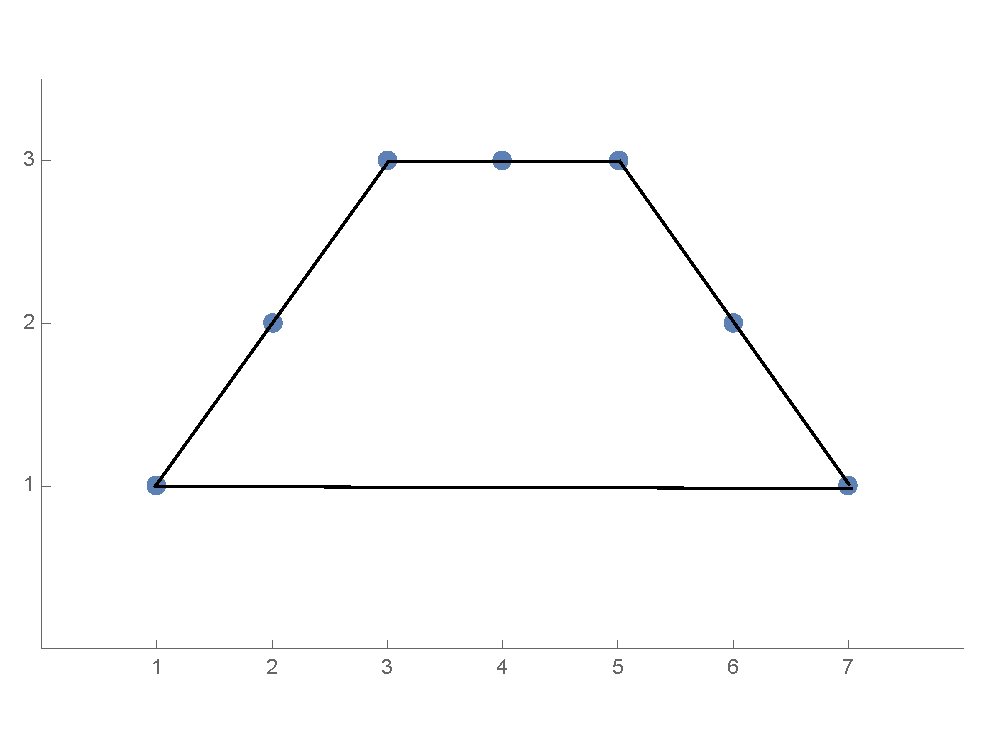
\includegraphics[width=3in]{Trapezoid73}
%\caption{Trapezoid associated to the Boolean function $\tau_{7,3}$}
%\label{trap73}
%\end{figure}
The opposite is also true, that is, for every isosceles trapezoid that can be constructed by steps of length at most 1, one can construct a trapezoid Boolean function. Trapezoid functions are very interesting
objects. Moreover, a handful of them seems to have special properties.  For example, a more general version of the trapezoid functions plays a central role in \cite{browncusick}.  Also, the trapezoid function
$\tau_{4,2}=X_1X_2+X_2X_3+X_3X_4$
is known to be a bent and negabent Boolean function \cite{parkerpott}.


It turns out that sequences of exponential sums of trapezoid Boolean functions of fixed degree satisfy homogeneous linear recurrences with integer coefficients.  These linear recurrences are the same ones satisfied by sequences of exponential sums of the rotation symmetric Boolean functions $R_{2,\cdots, k}(n)$.  Remarkably, this fact can be proved by elementary means by ``playing" a simple game of turning 
{\it ON} and {\it OFF} some of the variables.   Given a Boolean variable $X_i$, we say that it is turned {\it OFF} if $X_i$ assumes the value 0 and turned {\it ON} if the variable assumes the value 1.
In other words, each Boolean variable represents a ``switch" with two options: 0 ({\it OFF}) and 1 ({\it ON}).

We start the discussion with the recurrence for exponential sums of trapezoid Boolean functions.

\begin{theorem}
\label{trapezoidTHM}
 The sequence $\{S(\tau_{n,k})\}_{n=k}^\infty$ satisfies a homogeneous linear recurrence with integer coefficients whose characteristic polynomial is given by 
 \begin{equation}
 \label{charpoly}
  p_k(X)=X^k -2 (X^{k-2}+X^{k-3}+\cdots+X+1).
 \end{equation}
\end{theorem}
\begin{proof}
For the sake of simplicity, we present, in detail, the proof for the cases $k=3$ and $k=4$.  The general case becomes clear after that.  Moreover, the complete proof of a generalization of this theorem over any Galois field is presented in section \ref{anyGalois}.
 
Start with the case $k=3$.  Observe that by turning $X_n$ {\it OFF} and {\it ON} we get the identity
 \begin{equation}
 \label{firsttau}
  S(\tau_{n,3}) = S(\tau_{n-1,3})+S(\tau_{n-1,3}+X_{n-2}X_{n-1}).
 \end{equation}
Consider now $S(\tau_{n-1,3}+X_{n-2}X_{n-1})$.  Turn $X_{n-1}$ {\it OFF} and {\it ON} to get
\begin{equation}
\label{secondtau}
 S(\tau_{n-1,3}+X_{n-2}X_{n-1})=S(\tau_{n-2,3})+S(\tau_{n-2,3}+X_{n-2}+X_{n-3}X_{n-2}).
\end{equation}
Finally, turn $X_{n-2}$ {\it OFF} and {\it ON} to get
\begin{equation}
 S(\tau_{n-2,3}+X_{n-2}+X_{n-3}X_{n-2})=S(\tau_{n-3,3})-S(\tau_{n-3,3}+X_{n-3}+X_{n-4}X_{n-3}).
\end{equation}
The last equation is equivalent (after relabeling) to 
\begin{equation}
\label{thirdtau}
S(\tau_{n,3})=S(\tau_{n+1,3}+X_{n+1}+X_{n}X_{n+1})+S(\tau_{n,3}+X_{n}+X_{n-1}X_{n}).
\end{equation}

Observe that equations (\ref{firsttau}) and (\ref{secondtau}) can be combined to obtain
\begin{equation}
\label{fourthtau}
S(\tau_{n,3})=S(\tau_{n-1,3})+S(\tau_{n-2,3})+ S(\tau_{n-2,3}+X_{n-2}+X_{n-3}X_{n-2}).
\end{equation}
Let $a_{n,3} =S(\tau_{n,3}+X_{n}+X_{n-1}X_{n})$.  Note that (\ref{thirdtau}) implies that $S(\tau_{n,3})=a_{n+1,3}+a_{n,3}$.  Therefore, (\ref{fourthtau}) can be re-written as
\begin{eqnarray}
(a_{n+1,3}+a_{n,3}) = (a_{n,3}+a_{n-1,3})+(a_{n-1,3}+a_{n-2,3})+a_{n-2,3},
\end{eqnarray}
which is equivalent to 
\begin{equation}
a_{n+1,3} = 2a_{n-1,3}+2a_{n-2,3}.
\end{equation}
This implies that $\{a_{n,3}\}$ satisfies the linear recurrence whose characteristic polynomial is given by $p_3(X)$.  Since $S(\tau_{n,3})=a_{n+1,3}+a_{n,3}$, then $\{S(\tau_{n,3})\}$ also satisfies such recurrence and the result holds for $k=3$.

Consider now the case when $k=4$.  As was done in the case when $k=3$,  turning {\it OFF} and {\it ON} several variables leads to 
\begin{eqnarray}
\label{fifthtau}
S(\tau_{n,4})&=&S(\tau_{n-1,4})+S(\tau_{n-2,4})+S(\tau_{n-3,4})\\\nonumber
&&+S(\tau_{n-3,4}+X_{n-3}+X_{n-4}X_{n-3}+X_{n-5}X_{n-4}X_{n-3})
\end{eqnarray}
and
\begin{eqnarray}
S(\tau_{n,4})&=& S(\tau_{n+1,4}+X_{n+1}+X_{n}X_{n+1}+X_{n-1}X_{n}X_{n+1})\\\nonumber
&&+S(\tau_{n,4}+X_{n}+X_{n-1}X_{n}+X_{n-2}X_{n-1}X_{n}).
\end{eqnarray}
Now let $a_{n,4}=S(\tau_{n,4}+X_{n}+X_{n-1}X_{n}+X_{n-2}X_{n-1}X_{n})$ and observe that (\ref{fifthtau}) can be re-written as
\begin{equation}
(a_{n+1,4}+a_{n,4})=(a_{n,4}+a_{n-1,4})+(a_{n-1,4}+a_{n-2,4})+(a_{n-2,4}+a_{n-3,4})+a_{n-3,4},
\end{equation}
which is equivalent to
\begin{equation}
a_{n+1,4} = 2a_{n-1,4}+2a_{n-2,4}+2a_{n-3,4}.
\end{equation}
Therefore, $\{a_{n,4}\}$ satisfies the linear recurrence whose characteristic polynomial is given by $p_4(X)$.  Since $S(\tau_{n,4})=a_{n+1,4}+a_{n,4}$, then $\{S(\tau_{n,4})\}$ also satisfies such 
recurrence and the result also holds for $k=4$.  

In general, $S(\tau_{n,k})$ can be expressed as
\begin{align}
S(\tau_{n,k})&=\sum_{i=1}^{k-1} S(\tau_{n-i,k})+S\left(\tau_{n-k+1,k}+\sum_{j=0}^{k-2} \prod_{i=0}^j X_{n-k+1-i}\right)
\end{align}
and as
\begin{align}
S(\tau_{n,k})&=S\left(\tau_{n+1,k}+\sum_{j=0}^{k-2} \prod_{i=0}^j X_{n+1-i}\right)+S\left(\tau_{n,k}+\sum_{j=0}^{k-2} \prod_{i=0}^j X_{n-i}\right).
\end{align}
Combine these equations and proceed as before to obtain the result.  This concludes the proof.
\end{proof}

\begin{remark}
We point out that a more general version of Theorem \ref{trapezoidTHM} for cubic functions appears in \cite{browncusick}.
\end{remark}

It turns out that the sequence of exponential sums of $(1,2,\cdots,k)$-rotation symmetric Boolean functions, that is, of $R_{2,3,\cdots, k}(n)$, also satisfies the linear recurrence whose characteristic 
polynomial is the given $p_k(X)$. This is a well-known result for the case when $k=3$ (\cite{BCP,browncusick, cusickjohns}), but, to the knowledge of the area, the closed formula for the general case is new. 
%For simplicity, we denote the  $(1,2,\cdots,k)$-rotation symmetric Boolean function in $n$ variables by $\rho_{n,k}$.  For example,
%\begin{equation*}
% \rho_{6,4}=X_1 X_2 X_3 X_4+X_2 X_3 X_4 X_5+X_3X_4 X_5 X_6 +X_1 X_4 X_5 X_6+X_1 X_2 X_5 X_6+X_1 X_2 X_3 X_6.
%\end{equation*}
Before proving that $\{S(R_{2,3,\cdots, k}(n))\}$ satisfies the linear recurrence with characteristic polynomial $p_k(X)$, we show an auxiliary result which can be proved using the same arguments as in the 
proof of Theorem \ref{trapezoidTHM}.

\begin{lemma}
\label{trapezoidplusLemma}
 Let $\tau_{n,k}$ be the trapezoid Boolean function of degree $k$ in $n$ variables.  Suppose that $F({\bf X})$ is a Boolean polynomial in the first $j$ variables with $j<k$.  Then, the sequences
 $$\{S(\tau_{n,k}+F({\bf X}))\}$$ and $$\{S(\tau_{n,k}+F({\bf X})+X_n+X_nX_{n-1}+X_nX_{n-1}X_{n-2}+\cdots+X_nX_{n-1}\cdots X_{n-k+2})\}$$ satisfies the linear recurrence whose characteristic polynomial 
 is given by $p_k(X)$.
\end{lemma}

\begin{proof}
The proof of this result is almost identical to the proof of Theorem \ref{trapezoidTHM}.  We present it for the case when $k=4$ and $F({\bf X}) = X_1X_2+X_1X_2X_3$ in order
 to convince the reader that the proof follows almost verbatim.
 
As was done in the proof of Theorem \ref{trapezoidTHM}, by turning {\it OFF} and {\it ON} several variables one can obtain
 \begin{eqnarray}
\label{lemmatau}
\nonumber
S(\tau_{n,4}+F({\bf X}))&=&S(\tau_{n-1,4}+F({\bf X}))+S(\tau_{n-2,4}+F({\bf X}))+S(\tau_{n-3,4}+F({\bf X}))\\
&&+S(\tau_{n-3,4}+F({\bf X})+X_{n-3}+X_{n-4}X_{n-3}+X_{n-5}X_{n-4}X_{n-3})
\end{eqnarray}
and
\begin{eqnarray}
\label{lemmatau2}
S(\tau_{n,4}+F({\bf X}))&=& S(\tau_{n+1,4}+F({\bf X})+X_{n+1}+X_{n}X_{n+1}+X_{n-1}X_{n}X_{n+1})\\\nonumber
&&+S(\tau_{n,4}+F({\bf X})+X_{n}+X_{n-1}X_{n}+X_{n-2}X_{n-1}X_{n}).
\end{eqnarray}
Let $a_{n,4,F}=S(\tau_{n,4}+F({\bf X})+X_{n}+X_{n-1}X_{n}+X_{n-2}X_{n-1}X_{n})$ and use (\ref{lemmatau}) and (\ref{lemmatau2}) to get
\begin{equation}
a_{n+1,4,F} = 2a_{n-1,4,F}+2a_{n-2,4,F}+2a_{n-3,4,F}.
\end{equation}
Thus, $\{a_{n,4,F}\}$ satisfies the linear recurrence whose characteristic polynomial is $p_4(X)$.  Since $S(\tau_{n,4}+F({\bf X}))=a_{n+1,4,F}+a_{n,4,F}$, then $\{S(\tau_{n,4}+F({\bf X}))\}$ satisfies
the same recurrence and the result holds for this case.  This concludes the proof.
\end{proof}

Theorem \ref{trapezoidTHM} and Lemma \ref{trapezoidplusLemma} are all that is needed to show that the sequence of exponential sums of $R_{2,3,\cdots, k}(n)$ satisfies the linear
recurrence with characteristic polynomial $p_k(X)$.

\begin{theorem}
 The sequence $\{S(R_{2,3,\cdots, k}(n))\}$ satisfies the homogeneous linear recurrence whose characteristic polynomial is given by $p_k(X)$. 
\end{theorem}

\begin{proof}
 This result can also be proved by turning {\it OFF} and {\it ON} several variables.  As before, we provide the proof for the case when $k=4$.  The general case follows the same argument.
 
 To start the argument, turn {\it OFF} and {\it ON} the variable $X_n$ to get
 \begin{equation}
 \label{firstreduction}
  S(R_{2,3,4}(n)) = S(\tau_{n-1,4})+S(\tau_{n-1,4}+X_1X_2X_3+X_1X_2X_{n-1}+X_1X_{n-2}X_{n-1}+X_{n-3}X_{n-2}X_{n-1}).
 \end{equation}
Consider the second term of the right hand side of this equation.  Turn $X_{n-1}$ {\it OFF} and {\it ON} to get
\begin{align}
\label{secondterm2}
 S(\tau_{n-1,4}&+X_1X_2X_3+X_1X_2X_{n-1}+X_1X_{n-2}X_{n-1}+X_{n-3}X_{n-2}X_{n-1})\\\nonumber
 &=S(\tau_{n-2,4}+X_1X_2X_3)\\\nonumber
 &\,\,\,+S(\tau_{n-2,4}+X_1X_2+X_1X_2X_3+X_1X_{n-2}+X_{n-3}X_{n-2}+X_{n-4}X_{n-3}X_{n-2}).
\end{align}
Again, consider the second term of the right hand side of equation (\ref{secondterm2}). Turn $X_{n-2}$ {\it OFF} and {\it ON} to get
\begin{align}
\label{secondterm3}
 S(\tau_{n-2,4}&+X_1X_2+X_1X_2X_3+X_1X_{n-2}+X_{n-3}X_{n-2}+X_{n-4}X_{n-3}X_{n-2})\\\nonumber
 &=S(\tau_{n-3,4}+X_1X_2+X_1X_2X_3)\\\nonumber
 &\,\,\,+S(\tau_{n-3,4}+X_1+X_1X_2+X_1X_2X_3+X_{n-3}+X_{n-4}X_{n-3}+X_{n-5}X_{n-4}X_{n-3}).
\end{align}
Equations (\ref{firstreduction}), (\ref{secondterm2}) and (\ref{secondterm3}) lead to the equation
 \begin{align}
  S(R_{2,3,4}(n)) &= S(\tau_{n-1,4})+S(\tau_{n-2,4}+X_1X_2X_3)+S(\tau_{n-3,4}+X_1X_2+X_1X_2X_3)\\\nonumber
  & \,\,\,+S(\tau_{n-3,4}+X_1+X_1X_2+X_1X_2X_3+X_{n-3}+X_{n-4}X_{n-3}+X_{n-5}X_{n-4}X_{n-3}).
 \end{align}
Theorem \ref{trapezoidTHM} and Lemma \ref{trapezoidplusLemma} imply that $\{S(\tau_{n-1,4})\}$,  $\{S(\tau_{n-2,4}+X_1X_2X_3)\}$, $\{S(\tau_{n-3,4}+X_1X_2+X_1X_2X_3)\}$ and
$$\{S(\tau_{n-3,4}+X_1+X_1X_2+X_1X_2X_3+X_{n-3}+X_{n-4}X_{n-3}+X_{n-5}X_{n-4}X_{n-3})\}$$
satisfy the linear recurrence whose characteristic polynomial $p_4(X)$.  Since $\{S(R_{2,3,4}(n))\}$ is a linear combination of them, then the result holds when $k=4$.

In general, $S(R_{2,3,\cdots, k}(n))$ can be expressed as
\begin{align}
S(R_{2,3,\cdots, k}(n))&=S(\tau_{n-1,k})+\sum_{m=0}^{k-3} S\left(\tau_{n-2-m,k}+\sum_{j=0}^m \prod_{i=1}^{k-1-j} X_i\right)\\\nonumber
&\,\,\,+S\left(\tau_{n-k+1,k}+\sum_{j=1}^{k-1} \left(\prod_{i=1}^{j} X_i+ \prod_{i=0}^{j-1} X_{n-k+1-i}\right)\right)
%X_{n-k+1}+X_{n-k+1}X_{n-k}+\cdots+X_{n-k+1}X_{n-k}X_{n-k-1}\cdots X_{n-2k+3}\right)
\end{align}
Invoke Theorem \ref{trapezoidTHM} and Lemma \ref{trapezoidplusLemma} to get the result.  This concludes the proof.
\end{proof}

The same technique can be applied to find linear recurrences of exponential sums of other rotations.  Recall that 
\begin{equation}
R_{j_1,\cdots, j_s}(n)=X_1X_{j_1}\cdots X_{j_s}+X_2X_{j_1+1}\cdots X_{j_s+1}+\cdots+X_nX_{j_1-1}\cdots X_{j_s-1},
\end{equation}
where the indices are taken modulo $n$ and the complete system of residues is $\{1,2,\cdots, n\}$. 
%For instance, under this notation one has
%\begin{equation}
%\rho_{n,k}=R_{2,3,\cdots, k}(n).
%\end{equation}
We define the equivalent of the trapezoid Boolean function for $R_{j_1,\cdots, j_s}(n)$ as
\begin{equation}
T_{j_1,\cdots,j_s}(n)=X_1X_{j_1}\cdots X_{j_s}+X_2X_{j_1+1}\cdots X_{j_s+1}+\cdots+X_{n+1-j_s}X_{j_1+n-j_s}\cdots X_{j_{s-1}+n-j_s}X_n.
\end{equation}
For instance, under this notation one has
\begin{equation}
\tau_{n,k}=T_{2,3,\cdots, k}(n).
\end{equation}
It turns out that for $k\geq 4$, the sequences $\{S(R_{2,3,\cdots,k-2,k}(n))\}$ and $\{S(R_{2,3,\cdots,k-2,k+1}(n))\}$ both satisfy the linear recurrence whose characteristic polynomial is
\begin{equation}
q_k(X)=X^{k+1}-2X^{k-1}-2X^{k-2}-\cdots-2X^3-4.
\end{equation}
As just mentioned, this can be proved by playing a game of turning {\it ON} and {\it OFF} some variables.  However, the process becomes somewhat tedious at a very early stage.

Other examples on which this elementary method can be used to find explicit formulas for linear recurrences include the sequence
\begin{equation}
\{S(R_{2,3,\cdots,k}(n)+R_{2,3,\cdots,k-1}(n))\},
\end{equation}
which satisfies the linear recurrence with characteristic polynomial 
\begin{equation}
X^k-2X^{k-1}+2,
\end{equation}
the sequence
\begin{equation}
\{S(R_{2,3,\cdots, k-1,k}(n)+R_{2,3,\cdots,k-2,k}(n))\},
\end{equation}
which satisfies the linear recurrence with characteristic polynomial 
\begin{equation}
X^k-2X^{k-1}+2X-2,
\end{equation}
and the sequence 
\begin{equation}
\{S(R_{2, 3,\cdots, k-2,k}(n)+ R_{2, 3, \cdots, k-1}(n)+R_{2, 3, \cdots,k}(n))\},
\end{equation}
which satisfies the linear recurrence with characteristic polynomial 
\begin{equation}
X^k-2(X^{k-2}+X^{k-3}+\cdots+X^2+1).
\end{equation}
However, the process is somewhat tedious to be done by hand.  Automatization seems to be the way to go.  The reader is invited to read Cusick's work \cite{cusickArXiv}, which
includes {\em Mathematica} code that calculates a linear recurrence for the weights of a given rotation.

%%%%%%%%%%%%%%%%%%%%%%%%%%%%%%%%%%%%%%%%%%%%%%%%%%%%%%%%%%%%%%%%%%%
% Linear recurrences over Fq
%%%%%%%%%%%%%%%%%%%%%%%%%%%%%%%%%%%%%%%%%%%%%%%%%%%%%%%%%%%%%%%%%%%

\section{Linear recurrences over $\mathbb{F}_q$}
\label{anyGalois}

In this section we show that Cuscik's result is not unique to the Boolean case.  In fact, exponential sums over finite fields of rotation polynomials $R_{j_1,\cdots,j_s}(n)$ (and linear combination
of them) satisfy linear recurrences with constant coefficients.  This is a generalization of Cusick's result.

Consider the Galois field $\mathbb{F}_q = \{0,\alpha_1,\cdots,\alpha_{q-1}\}$ where $q=p^r$ with $p$ prime and $r\geq 1$.  The recall that the exponential sum
of a function $F:\mathbb{F}_q^n \to \mathbb{F}_q$ is given by
\begin{equation}
 S_{\mathbb{F}_q}(F)=\sum_{{\bf x}\in \mathbb{F}^n_q} e^{\frac{2\pi i}{p} \text{Tr}_{\mathbb{F}_q/\mathbb{F}_p}(F({\bf x}))},
\end{equation}
where $\text{Tr}_{\mathbb{F}_q/\mathbb{F}_p}$ represents the field trace function from $\mathbb{F}_q$ to $\mathbb{F}_p$.
The same technique used for exponential sums of Boolean functions can be used in general.  However, instead of having two options for the ``switch", we now have $q$ of them.  Let $X$ be a variable which takes values on $\mathbb{F}_q$.  As before, we say that the variable $X$ can be turned {\it OFF} or {\it ON}, however, this time the term ``turn {\it OFF}" means that $X$ assumes the value 0, while the term ``turn {\it ON}" means that $X$ assumes all values in $\mathbb{F}_q$ that are different from zero.  Think of this situation as a light switch on which you have the option to turn  {\it OFF} the light and the option to turn it {\it ON} to one of $q-1$ different colors.


We consider first sequences of exponential sums of trapezoid functions.  As in the Boolean case, they satisfy linear recurrences with integer coefficients over any Galois field 
$\mathbb{F}_q$.   We start with the following lemma, which is interesting in its own right.

\begin{lemma}
\label{generallemma}
Let $k, n$ and $j$ be integers with $k>2$, $1\leq j<k$ and $n\geq k$.   Then,
\begin{equation}
S_{\mathbb{F}_q}\left(T_{2,3,\cdots,k}(n)+\sum_{s=1}^j\beta_s\prod_{l=0}^{k-s-1}X_{n-l}\right)=S_{\mathbb{F}_q}\left(T_{2,3,\cdots,k}(n)+\sum_{s=1}^j\prod_{l=0}^{k-s-1}X_{n-l}\right)
\end{equation}
for any choice of $\beta_{s} \in \mathbb{F}_q^\times$.
\end{lemma}

\begin{proof}
The proof is by induction on $n$.  Suppose first that $n=k$.  Observe that
\begin{eqnarray}\nonumber
\label{basecase}
 T_{2,3,\cdots,k}(k)+\sum_{s=1}^j\beta_s\prod_{l=0}^{k-s-1}X_{k-l}&=& X_1X_2\cdots X_k+\beta_j X_{j+1}X_{j+2}\cdots X_k+\beta_{j-1} X_{j}X_{j+1}\cdots X_k\\
 &&+\cdots+ \beta_2 X_3 X_4\cdots X_k+  \beta_1 X_2 X_3\cdots X_k.
\end{eqnarray}
Consider the right hand side of (\ref{basecase}).  If $1\leq j\leq k-2$, then make the changes of variables
\begin{eqnarray*}
 X_t &=& Y_t, \,\,\, \text{ for }j+2\leq t \leq k \\
 X_{j+1}&=& \beta_j^{-1}Y_{j+1}\\
 X_t&=& \beta_{t-1}^{-1}\beta_t Y_t, \,\,\, \text{ for }2\leq t \leq j\\ 
 X_1&=& \beta_1 Y_1.
\end{eqnarray*}
On the other hand, if $j=k-1$, then make the change of variables
\begin{eqnarray*}
 X_{k}&=& \beta_{k-1}^{-1}Y_{k}\\
 X_t&=& \beta_{t-1}^{-1}\beta_t Y_t, \,\,\, \text{ for }2\leq t \leq k-1\\ 
 X_1&=& \beta_1 Y_1.
\end{eqnarray*}
This transforms (\ref{basecase}) into 
\begin{equation}
  Y_1Y_2\cdots Y_k +\sum_{s=1}^j\prod_{l=0}^{k-s-1}Y_{k-l}.
\end{equation}
Therefore, 
\begin{equation}
 S_{\mathbb{F}_q}\left(T_{2,3,\cdots,k}(k)+\sum_{s=1}^j\beta_s\prod_{l=0}^{k-s-1}X_{k-l}\right)=S_{\mathbb{F}_q}\left(T_{2,3,\cdots,k}(k)+\sum_{s=1}^j\prod_{l=0}^{k-s-1}X_{k-l}\right).
\end{equation}
This concludes the base case.  

Suppose now that for some $n\geq k$ we have 
\begin{equation}
 S_{\mathbb{F}_q}\left(T_{2,3,\cdots,k}(n)+\sum_{s=1}^j\beta_s\prod_{l=0}^{k-s-1}X_{n-l}\right)=S_{\mathbb{F}_q}\left(T_{2,3,\cdots,k}(n)+\sum_{s=1}^j\prod_{l=0}^{k-s-1}X_{n-l}\right).
\end{equation}
Consider 
\begin{equation}
 S_{\mathbb{F}_q}\left(T_{2,3,\cdots,k}(n+1)+\sum_{s=1}^j\beta_s\prod_{l=0}^{k-s-1}X_{n+1-l}\right).
\end{equation}
Suppose first that $1\leq j \leq k-2$.  Letting $X_{n+1}$ run over every element of the field leads to 
\begin{align}\nonumber
  S_{\mathbb{F}_q}(T_{2,3,\cdots,k}(n+1)+\sum_{s=1}^j\beta_s\prod_{l=0}^{k-s-1}X_{n+1-l}&)=S_{\mathbb{F}_q}\left(T_{2,3,\cdots,k}(n)\right)\\
  &+\sum_{\alpha\in\mathbb{F}_q^{\times}}  S_{\mathbb{F}_q}\left(T_{2,3,\cdots,k}(n)+\sum_{s=1}^{j+1}\gamma_s(\alpha)\prod_{l=0}^{k-s-1}X_{n-l}\right),
\end{align}
where $\gamma_1(\alpha)=\alpha$ and $\gamma_s(\alpha) = \alpha \beta_{s-1}$.  By induction
\begin{equation}
 S_{\mathbb{F}_q}\left(T_{2,3,\cdots,k}(n)+\sum_{s=1}^{j+1}\gamma_s(\alpha)\prod_{l=0}^{k-s-1}X_{n-l}\right)=S_{\mathbb{F}_q}\left(T_{2,3,\cdots,k}(n)+\sum_{s=1}^{j+1}\prod_{l=0}^{k-s-1}X_{n-l}\right).
\end{equation}
Therefore,
\begin{align}\nonumber
\label{indstep1}
  S_{\mathbb{F}_q}(T_{2,3,\cdots,k}(n+1)+\sum_{s=1}^j\beta_s\prod_{l=0}^{k-s-1}X_{n+1-l}&)= S_{\mathbb{F}_q}\left(T_{2,3,\cdots,k}(n)\right)\\
  &+\sum_{\alpha\in\mathbb{F}_q^{\times}}  S_{\mathbb{F}_q}\left(T_{2,3,\cdots,k}(n)+\sum_{s=1}^{j+1}\prod_{l=0}^{k-s-1}X_{n-l}\right).
\end{align}
However, (\ref{indstep1}) does not depend on the choice of the $\beta_t$'s. It follows that
\begin{align}\nonumber
  S_{\mathbb{F}_q}\left(T_{2,3,\cdots,k}(n+1)+\sum_{s=1}^j\beta_s\prod_{l=0}^{k-s-1}X_{n+1-l}\right)= S_{\mathbb{F}_q}\left(T_{2,3,\cdots,k}(n+1)+\sum_{s=1}^j\prod_{l=0}^{k-s-1}X_{n+1-l}\right)
\end{align}
is true for $1\leq j\leq k-2$.

Consider now the case $j=k-1$.  Again,  letting $X_{n+1}$ run over every element of the field leads to 
\begin{align}\nonumber
  S_{\mathbb{F}_q}(T_{2,3,\cdots,k}(n+1)&+\sum_{s=1}^{k-1}\beta_s\prod_{l=0}^{k-s-1}X_{n+1-l})= S_{\mathbb{F}_q}\left(T_{2,3,\cdots,k}(n)\right)\\
  &+\sum_{\alpha\in\mathbb{F}_q^{\times}} e^{\frac{2\pi i}{p} \text{Tr}_{\mathbb{F}_q/\mathbb{F}_p}(\alpha \beta_{k-1})} S_{\mathbb{F}_q}\left(T_{2,3,\cdots,k}(n)+\sum_{s=1}^{k-1}\gamma_s(\alpha)\prod_{l=0}^{k-s-1}X_{n-l}\right),
\end{align}
where $\gamma_1(\alpha)=\alpha$ and $\gamma_s(\alpha) = \alpha \beta_{s-1}$.  However, by induction
\begin{equation}
 S_{\mathbb{F}_q}\left(T_{2,3,\cdots,k}(n)+\sum_{s=1}^{k-1}\gamma_s(\alpha)\prod_{l=0}^{k-s-1}X_{n-l}\right)=S_{\mathbb{F}_q}\left(T_{2,3,\cdots,k}(n)+\sum_{s=1}^{j+1}\prod_{l=0}^{k-s-1}X_{n-l}\right).
\end{equation}
Since
\begin{equation}
 \sum_{\alpha \in \mathbb{F}_q^\times}e^{\frac{2\pi i}{p} \text{Tr}_{\mathbb{F}_q/\mathbb{F}_p}(\alpha \beta_{k-1})}=-1,
\end{equation}
then it follows that
\begin{align}\nonumber
\label{indstep2}
  S_{\mathbb{F}_q}(T_{2,3,\cdots,k}(n+1)+\sum_{s=1}^{k-1}\beta_s\prod_{l=0}^{k-s-1}X_{n+1-l}&)= S_{\mathbb{F}_q}\left(T_{2,3,\cdots,k}(n)\right)\\
  &- S_{\mathbb{F}_q}\left(T_{2,3,\cdots,k}(n)+\sum_{s=1}^{k-1}\prod_{l=0}^{k-s-1}X_{n-l}\right).
\end{align}
Since (\ref{indstep1}) does not depend on the choice of the $\beta_t$'s, then it follows that
\begin{eqnarray}\nonumber
  S_{\mathbb{F}_q}\left(T_{2,3,\cdots,k}(n+1)+\sum_{s=1}^{k-1}\beta_s\prod_{l=0}^{k-s-1}X_{n+1-l}\right)&=& S_{\mathbb{F}_q}\left(T_{2,3,\cdots,k}(n+1)+\sum_{s=1}^{k-1}\prod_{l=0}^{k-s-1}X_{n+1-l}\right)
\end{eqnarray}
is true.  This completes the induction and the proof.
\end{proof}

Next is the linear recurrence for exponential sums of trapezoid functions over any Galois field.

\begin{theorem}
\label{thmtrapgen}
Let $k\geq 2$ be an integer and $q=p^r$ with $p$ prime. The sequence $\{S_{\mathbb{F}_q}(T_{2,3,\cdots,k}(n))\}_{n=k}^\infty$ satisfies a homogeneous linear recurrence with integer coefficients whose characteristic polynomial is given by 
 \begin{equation}
 \label{charpolygeneral}
  Q_{T,k,\mathbb{F}_q}(X)=X^k-q \sum _{l=0}^{k-2} (q-1)^l X^{k-2-l}.
 \end{equation}
 In particular, when $q=2$ we recover Theorem \ref{trapezoidTHM}.
\end{theorem}

\begin{proof}
We present the proof for $k>2$.  The case $k=2$ can be proved using similar techniques.
 Start by turning $X_n$ {\it OFF} and {\it ON}, that is, by letting $X_n$ assume all its possible values.  This produces the identity
 \begin{eqnarray}
 \label{firstidgeneral}
  S_{\mathbb{F}_q}(T_{2,3,\cdots,k}(n))=S_{\mathbb{F}_q}(T_{2,3,\cdots,k}(n-1))+ \sum_{\beta \in \mathbb{F}_q^{\times}}S_{\mathbb{F}_q}\left(T_{2,3,\cdots,k}(n-1)+\beta \prod_{j=1}^{k-1} X_{n-j}\right)
 \end{eqnarray}
However, Lemma \ref{generallemma} implies
\begin{equation}
 S_{\mathbb{F}_q}\left(T_{2,3,\cdots,k}(n-1)+\beta \prod_{j=1}^{k-1} X_{n-j}\right)=S_{\mathbb{F}_q}\left(T_{2,3,\cdots,k}(n-1)+ \prod_{j=1}^{k-1} X_{n-j}\right)
\end{equation}
for every $\beta \in \mathbb{F}_q^{\times}$.  Therefore, (\ref{firstidgeneral}) reduces to 
 \begin{eqnarray}
 \label{secondidgeneral}
  S_{\mathbb{F}_q}(T_{2,3,\cdots,k}(n))=S_{\mathbb{F}_q}(T_{2,3,\cdots,k}(n-1))+ (q-1)S_{\mathbb{F}_q}\left(T_{2,3,\cdots,k}(n-1)+ \prod_{j=1}^{k-1} X_{n-j}\right)
 \end{eqnarray}
Consider now $S_{\mathbb{F}_q}\left(T_{2,3,\cdots,k}(n-1)+ \prod_{j=1}^{k-1} X_{n-j}\right)$. Let $X_{n-1}$ assume all its possible values and use the same argument as before to get
\begin{align}\nonumber
  S_{\mathbb{F}_q}(T_{2,3,\cdots,k}(n-1)+ \prod_{j=1}^{k-1} X_{n-j})&= \left(S_{\mathbb{F}_p} T_{2,3,\cdots,k}(n-2)\right)\\
 &+ (q-1) S_{\mathbb{F}_q}\left(T_{2,3,\cdots,k}(n-2)+\prod_{j=1}^{k-2} X_{n-1-j}+\prod_{j=1}^{k-1} X_{n-1-j}\right)
\end{align}
Thus, (\ref{secondidgeneral}) reduces to
\begin{eqnarray}\nonumber
 S_{\mathbb{F}_q}(T_{2,3,\cdots,k}(n))&=&S_{\mathbb{F}_q}(T_{2,3,\cdots,k}(n-1))+(q-1)S_{\mathbb{F}_q}\left(T_{2,3,\cdots,k}(n-2)\right)\\
 &+& (q-1)^2 S_{\mathbb{F}_q}\left(T_{2,3,\cdots,k}(n-2)+\prod_{j=1}^{k-2} X_{n-1-j}+\prod_{j=1}^{k-1} X_{n-1-j}\right).
\end{eqnarray}
Continue in this manner to get the following equation
\begin{eqnarray}
 \label{finalidgeneral}
 S_{\mathbb{F}_q}(T_{2,3,\cdots,k}(n))&=& \sum_{l=1}^{k-1}(q-1)^{l-1}S_{\mathbb{F}_q}T_{2,3,\cdots,k}(n-l))\\\nonumber
 &&+(q-1)^{k-1} S_{\mathbb{F}_q}\left(T_{2,3,\cdots,k}(n-k+1)+\sum_{j=0}^{k-2}\prod_{l=0}^j X_{n-k+1-l}\right).
\end{eqnarray}

On the other hand, let $X_{n+1}$ assume all its possible values and use Lemma \ref{generallemma} to get the equation
\begin{align}\nonumber
\label{axuliaryfinalgen}
S_{\mathbb{F}_q}(T_{2,3,\cdots,k}(n+1)+\sum_{j=0}^{k-2}\prod_{l=0}^j X_{n+1-l})&= S_{\mathbb{F}_q}(T_{2,3,\cdots,k}(n))\\
&+\sum_{\beta \in \mathbb{F}_q^{\times}}e^{\frac{2\pi i}{p}\text{Tr}_{\mathbb{F}_q/\mathbb{F}_p}(\beta)}S_{\mathbb{F}_q}\left(T_{2,3,\cdots,k}(n)+\sum_{j=0}^{k-2}\prod_{l=0}^j X_{n-l}\right).
%&&+e^{\frac{2\pi i}{p}\text{Tr}_{\mathbb{F}_q/\mathbb{F}_p}(\alpha_2)}S_{\mathbb{F}_q}\left(T_{2,3,\cdots,k}(n)+\sum_{j=0}^{k-2}\prod_{l=0}^j X_{n-l}\right)\\\nonumber
%&&+e^{\frac{2\pi i}{p}\text{Tr}_{\mathbb{F}_q/\mathbb{F}_p}(\alpha_3)}S_{\mathbb{F}_q}\left(T_{2,3,\cdots,k}(n)+\sum_{j=0}^{k-2}\prod_{l=0}^j X_{n-l}\right)\\\nonumber
%&&\vdots\\\nonumber
%&&+e^{\frac{2\pi i}{p}\text{Tr}_{\mathbb{F}_q/\mathbb{F}_p}(\alpha_{q-1})}S_{\mathbb{F}_q}\left(T_{2,3,\cdots,k}(n)+\sum_{j=0}^{k-2}\prod_{l=0}^j X_{n-l}\right).
\end{align}
Now use the well-known formula
\begin{equation}
\sum_{\beta\in\mathbb{F}_q^{\times}} e^{\frac{2\pi i}{p}\text{Tr}_{\mathbb{F}_q/\mathbb{F}_p}(\beta)}=-1.
\end{equation}  
to reduce (\ref{axuliaryfinalgen}) to 
\begin{align}
 S_{\mathbb{F}_q}(T_{2,3,\cdots,k}(n+1)+\sum_{j=0}^{k-2}\prod_{l=0}^j X_{n+1-l})&= S_{\mathbb{F}_q}(T_{2,3,\cdots,k}(n))\\\nonumber
 & - S_{\mathbb{F}_q}\left(T_{2,3,\cdots,k}(n)+\sum_{j=0}^{k-2}\prod_{l=0}^j X_{n-l}\right).
\end{align}
This last equation is equivalent to 
\begin{align}
\label{axuliaryfinalgen2}
 S_{\mathbb{F}_q}(T_{2,3,\cdots,k}(n))= S_{\mathbb{F}_q}(T_{2,3,\cdots,k}(n+1)&+\sum_{j=0}^{k-2}\prod_{l=0}^j X_{n+1-l})\\\nonumber
 & +S_{\mathbb{F}_q}\left(T_{2,3,\cdots,k}(n)+\sum_{j=0}^{k-2}\prod_{l=0}^j X_{n-l}\right).
\end{align}

Let $a_n = S_{\mathbb{F}_q}\left(T_{2,3,\cdots,k}(n)+\sum_{j=0}^{k-2}\prod_{l=0}^j X_{n-l}\right)$. Then,
\begin{equation}
 S_{\mathbb{F}_q}(T_{2,3,\cdots,k}(n))=a_{n+1}+a_n
\end{equation}
and equation (\ref{finalidgeneral}) is now
\begin{eqnarray}
 (a_{n+1}+a_n)&=&\sum_{l=1}^{k-1}(q-1)^{l-1}(a_{n+1-l}+a_{n-l})+(q-1)^{k-1} a_{n-k+1}.
\end{eqnarray}
The last equation reduces to
\begin{equation}
 a_{n+1}=\sum_{l=0}^{k-2} q(q-1)^{l}a_{n-1-l}
\end{equation}
This concludes the proof.
\end{proof}

The polynomial $Q_{T,k,\mathbb{F}_q}(X)$ is quite interesting. In particular, it seems to be irreducible for $k > 2$ and every $q=p^r$ with $p$ prime.  The irreducibility of $Q_{T,k,\mathbb{F}_q}(X)$ when $\gcd(k,r)=1$ 
is a consequence of the Eisenstein-Dumas criterion.

\begin{theorem}[Eisenstein-Dumas criterion]
Let $f(x)=a_n x^n+a_{n-1}x^{n-1}+\cdots+a_1 x+a_0 \in \mathbb{Z}[x]$ be a polynomial. Let $p$ be a prime. Denote the $p$-adic valuation of an integer $m$ by $\nu_p(m)$ (with $\nu_p(0)=+\infty$).  Suppose that
\begin{enumerate}
 \item $\nu_p(a_n)=0$,
 \item $\nu_p(a_{n-i})/i>\nu_p(a_0)/n$ for $1\leq i \leq n-1$, and
 \item $\gcd(\nu_p(a_0),n)=1$.
\end{enumerate}
Then, $f(x)$ is irreducible over $\mathbb{Q}$.
\end{theorem}

\begin{proposition}
 Let $q=p^r$ with $p$ prime.  Suppose that $\gcd(k,r)=1$.  Then, the polynomial
 \begin{equation}
  Q_{T,k,\mathbb{F}_q}(X)=X^k-q \sum _{l=0}^{k-2} (q-1)^l X^{k-2-l}
 \end{equation}
is irreducible over $\mathbb{Q}$.
\end{proposition}

\begin{proof}
 This is a direct consequence of the Eisenstein-Dumas criterion.
\end{proof}

Exponential sums over $\mathbb{F}_q$ of rotation functions $R_{2,\cdots,k}(n)$ also satisfy homogeneous linear recurrences.  However, in general, these linear recurrences have higher order than the 
homogeneous linear recurrences satisfied by exponential sums of trapezoid functions.  In other words, the identity observed over $\mathbb{F}_2$ between the linear recurrences of exponential sums of trapezoid Boolean functions and rotation symmetric Boolean functions is lost over $\mathbb{F}_q$.
For example, if we consider the monomial rotation 
\begin{equation}
 R_2(n)=X_1X_2+X_2X_3+\cdots+X_{n-1}X_n+X_nX_1,
\end{equation}
then we have the following result. 
\begin{theorem}
\label{thmrot2}
 Suppose that $p>2$ is prime.  Then, $\{S_{\mathbb{F}_p}(R_2(n)\}$ satisfy the homogeneous linear recurrence with characteristic polynomial 
 \begin{equation}
  Q_{R,2,\mathbb{F}_p}(X)=X^{4}-p^{2}.
 \end{equation}
\end{theorem}

\begin{proof}
This is the first result whose proof relies on linear algebra.  Turn $X_n$ and $X_{n-1}$ {\it OFF} and {\it ON}, that is, let them assume all values in $\mathbb{F}_p$, and use the identity
\begin{equation}
 S_{\mathbb{F}_p}(T_2(n)+\beta X_n) = S_{\mathbb{F}_p}(T_2(n)+ X_n), \text{ for }\beta\in\mathbb{F}_p^{\times}
\end{equation}
to get the equation 
\begin{eqnarray}
\label{rot2}
 S_{\mathbb{F}_p}(R_2(n))&=& S_{\mathbb{F}_p}(T_2(n-2))+(p-1)S_{\mathbb{F}_p}(T_2(n-2)+X_{n-2})\\\nonumber
 &&+\sum_{\alpha\in\mathbb{F}_p^\times}\sum_{\beta \in \mathbb{F}_p}e^{\frac{2\pi i}{p}\alpha\beta}S_{\mathbb{F}_p}(T_2(n-2)+\alpha X_1+\beta X_{n-2}),
\end{eqnarray}
Let 
\begin{eqnarray}
 a_0(n)&=&S_{\mathbb{F}_p}(T_2(n))\\\nonumber
 a_1(n)&=&S_{\mathbb{F}_p}(T_2(n)+X_n)\\\nonumber
 b_{\alpha,\beta}(n)&=&S_{\mathbb{F}_p}(T_2(n)+\alpha X_1+\beta X_n)\,\, \text{ for }\alpha\in\mathbb{F}_p^\times, \beta \in \mathbb{F}_p.
\end{eqnarray}
Then,
\begin{eqnarray}
 S_{\mathbb{F}_p}(R_2(n))&=& a_0(n-2)+(p-1)a_1(n-2)+\sum_{\alpha\in\mathbb{F}_p^\times}\sum_{\beta \in \mathbb{F}_p}e^{\frac{2\pi i}{p}\alpha\beta}b_{\alpha,\beta}(n-2).
\end{eqnarray}
Observe that
\begin{eqnarray}
 a_0(n)&=& a_0(n-1)+(p-1)a_1(n-1)\\\nonumber
 a_1(n)&=& a_0(n-1)-a_1(n-1)\\\nonumber
 b_{\alpha,\beta}(n)&=& \sum_{\gamma \in \mathbb{F}_p} e^{\frac{2\pi i}{p}(\beta \gamma)} b_{\alpha,\gamma}(n-1),
\end{eqnarray}
which can be written in matrix form as
\begin{equation}
 \left(
 \begin{array}{c}
 a_0(n)\\
 a_1(n)\\
 b_{1,0}(n)\\
 b_{1,1}(n)\\
 \vdots\\
 b_{p-1,p-1}(n)
 \end{array}
 \right)=A(p)\left(
 \begin{array}{c}
 a_0(n-1)\\
 a_1(n-1)\\
 b_{1,0}(n-1)\\
 b_{1,1}(n-1)\\
 \vdots\\
 b_{p-1,p-1}(n-1)
 \end{array}
 \right)
\end{equation}
where
\begin{eqnarray}
 A(p)&=\left(
\begin{array}{c|c|c|c|c}
 A_0(p)& O & O  &\cdots & O\\
 \hline
 O & A_1(p) & O &\cdots & O\\
 \hline
  O & O & A_2(p) &\cdots & O\\
  \hline
\vdots & \vdots & \vdots &\ddots & \vdots\\
\hline
  O & O & O &\cdots & A_{p-1}(p)\\
\end{array}
\right),
\end{eqnarray}
and
\begin{equation}
\label{DFT}
A_0(p)=\left(
\begin{array}{cc}
1 & p-1\\
 1 & -1 \\
 \end{array}\right)\,\,\,\, \text{ and } \,\,\,\,A_{j}(p) = \left(
\begin{array}{ccccc}
 1 & 1 & 1 & \cdots & 1 \\
 1 & e^{\frac{2  \pi i}{p}} & e^{\frac{4  \pi i}{p}}& \cdots & e^{\frac{2(p-1)\pi i}{p}} \\
  1 & e^{\frac{4   \pi i}{p}} & e^{\frac{8 \pi i}{p}}& \cdots & e^{\frac{2\times 2(p-1)\pi i}{p}} \\
 \vdots & \vdots & \vdots&  \ddots & \vdots \\
  1 & e^{\frac{2(p-1) \pi i}{p}} & e^{\frac{4(p-1) \pi i}{p}}& \cdots & e^{\frac{2\times (p-1)^2\pi i}{p}} \\
\end{array}
\right), 
\end{equation}
for $1\leq j \leq p-1.$
It is clear that the first block $A_0(p)$ satisfies $X^2-p$.  All other blocks $A_j(p)$'s, for $1\leq j \leq p-1$, are $\sqrt{p}\cdot W_p$, where $W_p$ is the $p\times p$ square Discrete Fourier 
Transform matrix.
Observe that
\begin{equation}
 A_j(p)^2 = \left(
\begin{array}{ccccc}
 p & 0 & \cdots & 0 & 0 \\
 0 & 0 & \cdots & 0 & p \\
 0 & 0 & \cdots & p & 0 \\
 \vdots & \vdots & \Ddots & \vdots & \vdots \\
 0 & p & \cdots & 0 & 0 \\
\end{array}
\right).
\end{equation}
Therefore,
\begin{equation}
A_j(p)^4 = \left(
\begin{array}{ccccc}
 p^2 & 0 & 0 &  \cdots & 0 \\
 0 & p^2 & 0 & \cdots & 0 \\
 0 & 0 & p^2 &\cdots & 0 \\
 \vdots & \vdots & \vdots & \ddots & \vdots \\
 0 & 0 & 0 &\cdots  & p^2 \\
\end{array}
\right).
\end{equation}
where $I_p$ represents the $p\times p$ identity matrix.  In other words, the big blocks $A_j(p)$'s satisfy $X^4-p^2$.  Since $X^2-p\,|\, X^4-p^2$, then we conclude that the matrix $A(p)$ satisfies the polynomial
 \begin{equation}
  Q_{R,2,\mathbb{F}_p}(X)=X^{4}-p^{2}. 
 \end{equation}
This means that the sequences $\{a_0(n)\}$, $\{a_1(n)\}$ and $\{b_{\alpha,\beta}(n)\}$, for $\alpha \in\mathbb{F}_p^\times,\beta \in \mathbb{F}_p$, all satisfy the linear
recurrence with characteristic polynomial given by $Q_{R,2,\mathbb{F}_p}(X)$.  Since $\{S_{\mathbb{F}_p}(R_2(n))\}$ is a combination of these sequences, then it also satisfies this recurrence.
This concludes the proof.
\end{proof}

We are now ready to prove one of the main results of this chapter.  That is, exponential sums of $R_{2,\cdots,k}(n)$ satisfy linear recurrences with integer coefficients.

\begin{theorem}
\label{generalTHM}
 Let $k\geq 2$ be an integer and $q=p^r$ with $p$ prime and $r\geq 1$.  The sequence $\{S_{\mathbb{F}_q}(R_{2,3,\cdots,k}(n))\}_{n\geq k}$ satisfies a linear recurrence with integer coefficients.
\end{theorem}

\begin{proof}
 Let $\zeta_p=e^{2\pi i/p}$. Consider the expression $S_{\mathbb{F}_q}(R_{2,3,\cdots, k}(n+k))$.  Let $X_{n+k}, X_{n+k-1}, \cdots,\\ X_{n+1}$ assume all values in $\mathbb{F}_q$ and observe that $S_{\mathbb{F}_q}(R_{2,3,\cdots, k}(n+k))$
 can be written as a linear combination of expressions of the form
 \begin{equation}
 \label{generatingseqs}
  a_{\boldsymbol{\alpha};\boldsymbol{\beta}}(n)=S_{\mathbb{F}_q}\left(T_{2,3,\cdots, k}(n)+\sum _{j=1}^{k-1} \left(\alpha _j \prod _{l=1}^j X_{n+1-l}+\beta _j \prod _{l=1}^j X_l\right)\right),
 \end{equation}
 where $\boldsymbol{\alpha}=(\alpha_1,\cdots,\alpha_{k-1}) \in \mathbb{F}_q^{k-1}$ and $\boldsymbol{\beta}=(\beta_1,\cdots,\beta_{k-1}) \in \mathbb{F}_q^{k-1}$.
Moreover, note that for each $\boldsymbol{\alpha},\boldsymbol{\beta} \in \mathbb{F}_q^{k-1}$, we have
 \begin{equation}
 \label{lineareqs}
  a_{\boldsymbol{\alpha};\boldsymbol{\beta}}(n) = \sum_{\boldsymbol{\gamma},\boldsymbol{\lambda}\in \mathbb{F}_q^{k-1}}c_{\boldsymbol{\gamma},\boldsymbol{\lambda}}\cdot a_{\boldsymbol{\gamma},\boldsymbol{\lambda}}(n-1),
 \end{equation}
where $c_{\boldsymbol{\gamma},\boldsymbol{\lambda}} \in \mathbb{Z}[\zeta_p]$ is a cyclotomic integer.  Let $A_{2,3,\cdots, k}(q)$ be the corresponding matrix for the linear equations in (\ref{lineareqs}) and
$F(X)$ be some annihilating polynomial for $A_{2,3,\cdots, k}(q)$.   We can assume that $F(X)$ has integer coefficients.  This is because the minimal polynomial of $A_{2,3,\cdots,k}(q)$ is monic, 
has algebraic integers coefficients and integrality is transitive.  In other words, if $m(X)$ is the minimal polynomial of $A_{2,3,\cdots,k}(q)$, then there is a polynomial with integer coefficients $F(X)$ 
such that $m(x)$ divides $F(X)$.  This polynomial $F(X)$ is an annihilating polynomial for $A_{2,3,\cdots,k}(q)$.

Each $\{a_{\boldsymbol{\alpha};\boldsymbol{\beta}}(n)\}_n$ satisfies the linear recurrence with characteristic polynomial given
by $F(X)$. Since $\{S_{\mathbb{F}_q}(R_{2,3,\cdots, k}(n+k))\}$ is a linear combination of these sequences, then $\{S_{\mathbb{F}_q}(R_{2,3,\cdots, k}(n+k))\}$ also satisfies such recurrence.
This concludes the proof.
\end{proof}


\begin{definition}
Let $\{b(n)\}$ be a sequence on an integral domain $D$.  A set of sequences $$\{\{a_1(n)\}, \{a_2(n)\},\cdots, \{a_s(n)\}\},$$ where $s$ is some natural number, is called a 
{\em recursive generating set for} $\{b(n)\}$ if 
\begin{enumerate}
 \item there is an integer $l$ such that for every $n$, $b(n)$ can be written as a linear combination of the form 
 $$b(n)=\sum_{j=1}^s c_j\cdot a_j(n-l),$$  
 where $c_j$'s are constants that belong to $D$, and
 \item for each $1\leq j_0 \leq s$ and every $n$, $a_{j_0}(n)$ can be written as a linear combination of the form 
 $$a_{j_0}(n)=\sum_{j=1}^s d_j\cdot a_j(n-1),$$
 where $d_j$'s are also constants that belong to $D$.
\end{enumerate}
The sequences $\{a_j(n)\}$'s are called {\it recursive generating sequences for} $\{b(n)\}$.
\end{definition}


\begin{remark}
It is a well-known result in the theory of recursive sequences that a sequence that has a recursive generating set satisfies a linear recurrence with constant coefficients.  In fact, this technique has been used in Theorems \ref{thmrot2} and \ref{generalTHM}.
\end{remark}

Theorem \ref{generalTHM} can be generalized to monomial rotation functions of the form $$R_{j_1,\cdots, j_s}(n)$$, for integers $j_0=1<j_1<\cdots <j_s$, and linear combinations of them.  Consider
\begin{align*}
 S_{\mathbb{F}_q}(R_{j_1,\cdots,j_s}(n+j_s)).
\end{align*} 
Observe that 
\begin{align*}
R_{j_1,\cdots,j_s}(n+j_s)=T_{j_1,\cdots,j_s}&(n)+X_{n+1}X_{n+j_1}\cdots X_{n+j_s}\\&+\sum _{m=0}^{s-1}\,\, \sum _{l=j_s-j_{m+1}+1}^{j_s-j_m} \left(\prod _{i=0}^m
   X_{j_i+l+n} \prod _{i=m+1}^s X_{j_i-j_s+l}+\prod _{i=0}^s
   X_{j_i-j_s+l+n} \right).
\end{align*}
Therefore, by turning {\it OFF} and {\it ON} the variables $X_{n+j_s},\cdots,X_{n+j_1}, X_{n+j_0}$ we can express $S_{\mathbb{F}_q}(R_{j_1,\cdots,j_s}(n+j_s))$ as a linear combination of terms $a_{\boldsymbol{\alpha},\boldsymbol{\beta}}(n)$ similar to (\ref{generatingseqs}).  In fact, the equivalent of the sequence in the argument of $S_{\mathbb{F}_q}(\,\cdot\,)$ in (\ref{generatingseqs}) is the trapezoid $T_{j_1,\cdots,j_s}(n)$
plus $2(j_s-1)$ terms of lower degree, similar to what happened in (\ref{generatingseqs}).  The set 
$$\{\{a_{\boldsymbol{\alpha},\boldsymbol{\beta}}(n)\}\}_{\boldsymbol{\alpha},\boldsymbol{\beta}\in \mathbb{F}_{q}^{j_s-1}}$$ turns out to be a recursive generating set and therefore
the sequence $\{R_{j_1,\cdots, j_s}(n)\}$ satisfies a linear recurrence with constant coefficients.  As in Theorem \ref{generalTHM}, it can be argued that a linear recurrence with 
integer coefficients is guaranteed to exist.  The argument for linear combinations of monomial rotation functions $R_{j_1,\cdots, j_s}(n)$ is very similar.

As an example of this discussion, consider the sequence $\{S_{\mathbb{F}_q}(R_{2,4,5}(n+5))\}$.  Turning {\it OFF} and {\it ON} the variables $X_{n+5},\cdots,X_{n+1}$, the exponential 
sum $S_{\mathbb{F}_q}(R_{2,4,5}(n+5))$ can be expressed as linear combination of terms of the form
\begin{align*}
 a_{\boldsymbol{\alpha},\boldsymbol{\beta}}(n)=S_{\mathbb{F}_q}(T_{2,4,5}(n)&+\alpha _1 X_1+\alpha _2 X_1 X_2+\alpha _3 X_2 X_3+\alpha _4X_1 X_3 X_4\\
 &+\beta _1 X_{n-2} X_{n-1}+\beta _2 X_n+\beta _3 X_{n-3} X_{n-2} X_n+\beta _4X_{n-1} X_n)
\end{align*}
For each $\boldsymbol{\alpha},\boldsymbol{\beta} \in \mathbb{F}_q^{4}$, we have
$$a_{\boldsymbol{\alpha},\boldsymbol{\beta}}(n)=\sum_{\boldsymbol{\gamma},\boldsymbol{\lambda} \in\mathbb{F}_q^{4}} c_{\boldsymbol{\gamma},\boldsymbol{\lambda}}a_{\boldsymbol{\gamma},\boldsymbol{\lambda}}(n-1),$$
where $c_{\boldsymbol{\gamma},\boldsymbol{\lambda}} \in \mathbb{Z}[\zeta_p]$, where $\zeta_p = e^{2\pi i/p}$.  Thus, $\{S_{\mathbb{F}_q}(R_{2,4,5}(n))\}$ satisfies a linear recurrence with integer coefficients.
All this information is summarized in the following theorem.

\begin{theorem}
 Let $p$ be prime and $q=p^r$.  Consider the function 
 $$F_n = \sum_{t=1}^N \beta_t R_{j_{t,1},\cdots, j_{t,s_t}}(n),$$
 where $\beta_t\in \mathbb{F}_q$ and $1<j_{t,1}<\cdots<j_{t,s_t}$ are integers.  The sequence $\{S_{\mathbb{F}_q}(F_n)\}$ satisfies a linear recurrence with integer coefficients.
\end{theorem}

%%%%%%%%%%%%%%%%%%%%%%%%%%%%%%%%%%%%%%%%%%%%%%%%%%%%%%%%%%%%%%%%%%%%%
% Symmetric Polynomials
%%%%%%%%%%%%%%%%%%%%%%%%%%%%%%%%%%%%%%%%%%%%%%%%%%%%%%%%%%%%%%%%%%%%%

\section{Linear recurrences over $\mathbb{F}_q$: Symmetric polynomials case}
\label{symmetriccase}

The method of turning {\it OFF} and {\it ON} is very elementary, but quite powerful.  For instance, it can also be used to prove that exponential sums over Galois fields of elementary symmetric polynomials (and linear combinations of them) satisfy homogeneous linear
recurrences with integer coefficients.  This was already hinted by the Boolean case, which is already known, that is, exponential sums of symmetric Boolean functions are linear recurrent.  This was first 
established by Cai, Green and Thierauf \cite{cai} and was used in \cite{cm1} to show that a conjecture of Cusick, Li and St$\check{\mbox{a}}$nic$\check{\mbox{a}}$ \cite{cusick2} is true asymptotically.  In \cite{cm2}, some of the results of 
\cite{cm1} where extended to some perturbations of symmetric Boolean functions.  This recursivity was also used in \cite{cm3, cusick4} to study the periodicity mod $p$ ($p$ prime) of exponential sums of 
symmetric Boolean functions. 

Let $\boldsymbol{e}_{n,k}$ be the elementary symmetric polynomial in $n$ variables of degree $k$. For example,
\begin{equation}
\boldsymbol{e}_{4,3} = X_1 X_2 X_3+X_1 X_4 X_3+X_2 X_4 X_3+X_1 X_2 X_4.
\end{equation}

We have the following result.

\begin{theorem}
\label{MoregeneralTHMSymmetric}
 Let $k\geq 2$ be an integer and $q=p^r$ with $p$ prime and $r\geq 1$.  The sequence 
\begin{equation}
\left\{ S_{\mathbb{F}_q}\left(\sum _{j=0}^{k-1} \beta_j \boldsymbol{e}_{n,k-j}\right)\right\}
\end{equation}
satisfies a linear recurrence with constant coefficients, regardless of the choice of the $\beta_j$'s.
\end{theorem}

\begin{proof}
We present the proof for $\{S_{\mathbb{F}_q}(\boldsymbol{e}_{n,k}\}$.  The general proof follows the same argument. Consider the expression $S_{\mathbb{F}_q}(\boldsymbol{e}_{n+k,k})$.  Define
\begin{equation}
 \label{generatingseqsSym}
  a_{\boldsymbol{\beta}}(n)=S_{\mathbb{F}_q}\left(\boldsymbol{e}_{n,k}+\sum _{j=1}^{k-1} \beta_j \boldsymbol{e}_{n,k-j}\right),
 \end{equation}
The set $\{\{a_{\boldsymbol{\beta}}(n)\}\}_{\boldsymbol{\beta}\in \mathbb{F}_q^{k-1}}$ is a recursive generating set for $\{S_{\mathbb{F}_q}(\boldsymbol{e}_{n+k,k}\}$.  Therefore, the sequence 
$\{S_{\mathbb{F}_q}(\boldsymbol{e}_{n+k,k}\}_{n\geq k}$ satisfies a linear recurrence with constant coefficients.  As in the proof of Theorem \ref{generalTHM}, it can be argued that a linear recurrence with 
integer coefficients is guaranteed to exist.  This concludes the proof.
\end{proof}

\begin{example}
Consider the sequence $\{S_{\mathbb{F}_3}(\boldsymbol{e}_{n,3}\}$.  Recall that in this case the generating sequences are given by 
 \begin{equation}
  a_{(s,t)}(n)=\{S_{\mathbb{F}_3}(\boldsymbol{e}_{n,3}+s\boldsymbol{e}_{n,2}+t\boldsymbol{e}_{n,1}\},
 \end{equation}
 where $s,t\in \mathbb{F}_3$.  Establish the order
 $$(0,0), (1,0), (2,0), (0,1), (1,1), (2,1), (0,2),(1,2), (2,2).$$
 Then, 
 \begin{equation}
\left( \begin{array}{c}
  a_{(0,0)}(n)\\
  a_{(1,0)}(n)\\
  \vdots\\
  a_{(2,2)}(n)
 \end{array}
\right) = A \left( \begin{array}{c}
  a_{(0,0)}(n-1)\\
  a_{(1,0)}(n-1)\\
  \vdots\\
  a_{(2,2)}(n-1)
 \end{array}
\right),
\end{equation}
where the matrix $A$ is given by
\begin{equation}
 A=\left(
\begin{array}{ccccccccc}
 1 & 1 & 1 & 0 & 0 & 0 & 0 & 0 & 0 \\
 0 & 1 & 0 & 0 & 0 & 1 & 1 & 0 & 0 \\
 0 & 0 & 1 & 0 & 1 & 0 & 1 & 0 & 0 \\
 0 & 0 & 0 & 1 & e^{\frac{2 i \pi }{3}} & e^{-\frac{2 i \pi }{3}} & 0 & 0 & 0 \\
 e^{-\frac{2 i \pi }{3}} & 0 & 0 & 0 & 1 & 0 & 0 & 0 & e^{\frac{2 i \pi }{3}} \\
 e^{\frac{2 i \pi }{3}} & 0 & 0 & 0 & 0 & 1 & 0 & e^{-\frac{2 i \pi }{3}} & 0 \\
 0 & 0 & 0 & 0 & 0 & 0 & 1 & e^{-\frac{2 i \pi }{3}} & e^{\frac{2 i \pi }{3}} \\
 0 & 0 & e^{-\frac{2 i \pi }{3}} & e^{\frac{2 i \pi }{3}} & 0 & 0 & 0 & 1 & 0 \\
 0 & e^{\frac{2 i \pi }{3}} & 0 & e^{-\frac{2 i \pi }{3}} & 0 & 0 & 0 & 0 & 1 \\
\end{array}
\right).
\end{equation}
\end{example}

We will not go into more details with elementary symmetric polynomials because the discussion does not bring anything new.  We will, however, consider the quadratic case because we consider it fascinating.
Moreover, we can calculate the spectrum of the corresponding matrix.

%%%%%%%%%%%%%%%%%%%%%%%%%
%Inicio del cambio
%%%%%%%%%%%%%%%%%%%%%%%%%


%%%%%%%%%%%%%%%%%%%%%%%%%%%%%%%%%%%%%%%%%%%%%%%%%%%%%%%%%%%%%%%%%%%%%
% Se aniquila el siguiente parrafo (version del articulo) para cambiarlo por la versio original (preprint) La secuencia es que ingreso la version original y despues el parrafo aniquilada
%%%%%%%%%%%%%%%%%%%%%%%%%%%%%%%%%%%%%%%%%%%%%%%%%%%%%%%%%%%%%%%%%%%%%

% Observe that the collection of sequences
% \begin{equation}
% \{a_{s}(n)\} = \{S_{\mathbb{F}_p}(\boldsymbol{e}_{n,2}+s\boldsymbol{e}_{n,1})\},
% \end{equation}
%where $s\in \mathbb{F}_p$, is a recursive generating set for $\{S_{\mathbb{F}_p}(\boldsymbol{e}_{n,2})\}$.  Also,
%\begin{equation}
%\left( \begin{array}{c}
%  a_0(n)\\
%  a_1(n)\\
%  \vdots\\
%  a_{p-1}(n)
% \end{array}
%\right) = M(p) \left( \begin{array}{c}
%  a_0(n-1)\\
%  a_1(n-1)\\
%  \vdots\\
%  a_{p-1}(n-1)
% \end{array}
%\right),
%\end{equation}
%where the matrix $M(p)$ %is given by
%\begin{equation}
%M(p)=\left(\begin{array}{ccccccc}
%1 & 1 & 1 & 1& 1 & \cdots & 1 \\
%e^{\frac{2(p-1)\pi i}{p}} & 1 & e^{\frac{2 \pi i}{p}} & e^{\frac{4 \pi i}{p}} & e^{\frac{6 \pi i}{p}}& \cdots & e^{\frac{2(p-2)\pi i}{p}}\\
%e^{\frac{2\times 2(p-2)\pi i}{p}}& e^{\frac{2\times 2(p-1)\pi i}{p}} & 1 & e^{\frac{4  \pi i}{p}} & e^{\frac{8 \pi i}{p}}& \cdots & e^{\frac{2\times 2(p-3)\pi i}{p}} \\
%e^{\frac{2\times 3(p-3)\pi i}{p}}& e^{\frac{2\times 3(p-2)\pi i}{p}} & e^{\frac{2\times 3(p-1)\pi i}{p}} & 1 & e^{\frac{6  \pi i}{p}} &  \cdots & e^{\frac{2\times 2(p-3)\pi i}{p}} \\
%e^{\frac{2\times 4(p-4)\pi i}{p}}& e^{\frac{2\times 4(p-3)\pi i}{p}} & e^{\frac{2\times 4(p-2)\pi i}{p}} & e^{\frac{2\times 4(p-2)\pi i}{p}} &  1 &   \cdots & e^{\frac{2\times 2(p-3)\pi i}{p}} \\
 %\vdots& \vdots& \vdots & \vdots & \vdots& \ddots & \vdots \\
%e^{\frac{2(p-1) \pi i}{p}} & e^{\frac{2\times 2(p-1) \pi i}{p}}  & e^{\frac{2\times 3(p-1) \pi i}{p}} & e^{\frac{2\times 4(p-1) \pi i}{p}} & e^{\frac{2\times 5 (p-1)\pi i}{p}}  & \cdots & 1 \\
 %\end{array}\right).
%\end{equation}
%The matrix $M(p)$ 
%can be obtained from the $p\times p$ Fourier Discrete Transform Matrix by replacing its $j$-row ${\bf r}_j$ by $RTC^{j-1}({\bf r}_j)$, where $RTC$ is the {\it rotate through carry}
%function
%\begin{equation}
% RTC(a_1,a_2,a_3,\cdots, a_n) = (a_n,a_1,a_2,\cdots, a_{n-1})
%\end{equation}
%and $RTC^m$ represents $m$ iterations of $RTC$.  In other words, the matrix $M(p)$ has $(j,k)$-entry $\zeta_p^{j(k-j)}$
% where $\zeta_p= \exp(2\pi i/p)$ and $j$ and $k$ run from $0$ to $p-1$ inclusive.
%It is not hard to prove that $M(p)$ is a Complex Hadamard Matrix.  In particular,
%\begin{equation}
%M(p) \overline{M(p)}^T = \overline{M(p)}^T M(p) = pI_p,
%\end{equation}
%where $I_p$ represents the $p\times p$ identity matrix.
%This implies that $M(p)$ is diagonalizable and that all its eigenvalues satisfy $|\lambda|=\sqrt{p}$.  Moreover, its eigenvalues are related to $g(a;p)$, the number-theoretical quadratic Gauss sum mod $p$ .  It is well-established that
%\begin{equation}
%\label{gaussvalue}
%g(a;p) = \left(\frac{a}{p}\right)g(1;p)\,\,\, \text{ and }\,\,\, g(1;p) = \begin{cases}
% \sqrt{p} & p\equiv 1 \mod 4 \\
% i\sqrt{p} & p\equiv 3 \mod 4.
%\end{cases}
%\end{equation}
%where $(a/p)$ denotes the Legendre's symbol.

\subsection{Quadratic case}
The case of the elementary symmetric polynomial of degree 2 is fascinating.  Observe that
 \begin{equation}
  a_{s}(n) = S_{\mathbb{F}_p}(\boldsymbol{e}_{n,2}+s\boldsymbol{e}_{n,1}),
 \end{equation}
where $s\in \mathbb{F}_p$, are the generating sequences of $\{S_{\mathbb{F}_p}(\boldsymbol{e}_{n,2})\}$.  Also,
\begin{equation}
\left( \begin{array}{c}
  a_0(n)\\
  a_1(n)\\
  \vdots\\
  a_{p-1}(n)
 \end{array}
\right) = M(p) \left( \begin{array}{c}
  a_0(n-1)\\
  a_1(n-1)\\
  \vdots\\
  a_{p-1}(n-1)
 \end{array}
\right),
\end{equation}
where the matrix $M(p)$ is given by
\begin{equation}
M(p)=\left(\begin{array}{ccccccc}
1 & 1 & 1 & 1& 1 & \cdots & 1 \\
e^{\frac{2(p-1)\pi i}{p}} & 1 & e^{\frac{2 \pi i}{p}} & e^{\frac{4 \pi i}{p}} & e^{\frac{6 \pi i}{p}}& \cdots & e^{\frac{2(p-2)\pi i}{p}}\\
e^{\frac{2\times 2(p-2)\pi i}{p}}& e^{\frac{2\times 2(p-1)\pi i}{p}} & 1 & e^{\frac{4  \pi i}{p}} & e^{\frac{8 \pi i}{p}}& \cdots & e^{\frac{2\times 2(p-3)\pi i}{p}} \\
e^{\frac{2\times 3(p-3)\pi i}{p}}& e^{\frac{2\times 3(p-2)\pi i}{p}} & e^{\frac{2\times 3(p-1)\pi i}{p}} & 1 & e^{\frac{6  \pi i}{p}} &  \cdots & e^{\frac{2\times 2(p-3)\pi i}{p}} \\
e^{\frac{2\times 4(p-4)\pi i}{p}}& e^{\frac{2\times 4(p-3)\pi i}{p}} & e^{\frac{2\times 4(p-2)\pi i}{p}} & e^{\frac{2\times 4(p-2)\pi i}{p}} &  1 &   \cdots & e^{\frac{2\times 2(p-3)\pi i}{p}} \\
 \vdots& \vdots& \vdots & \vdots & \vdots& \ddots & \vdots \\
e^{\frac{2(p-1) \pi i}{p}} & e^{\frac{2\times 2(p-1) \pi i}{p}}  & e^{\frac{2\times 3(p-1) \pi i}{p}} & e^{\frac{2\times 4(p-1) \pi i}{p}} & e^{\frac{2\times 5 (p-1)\pi i}{p}}  & \cdots & 1 \\
 \end{array}\right).
\end{equation}
The matrix $M(p)$ can be obtained from the $p\times p$ Fourier Discrete Transform Matrix by replacing its $j$-row ${\bf r}_j$ by $RTC^{j-1}({\bf r}_j)$, where $RTC$ is the {\it rotate through carry}
function
\begin{equation}
 RTC(a_1,a_2,a_3,\cdots, a_n) = (a_n,a_1,a_2,\cdots, a_{n-1})
\end{equation}
and $RTC^m$ represents $m$ iterations of $RTC$.


It is not hard to prove that $M(p)$ is a Complex Hadamard Matrix.  In particular,
\begin{equation}
M(p) \overline{M(p)}^T = \overline{M(p)}^T M(p) = \left(
\begin{array}{ccccc}
  p & 0 & 0 & \cdots & 0 \\
 0 & p & 0 & \cdots & 0 \\
 0 & 0 &p & \cdots & 0 \\
 \vdots & \vdots & \vdots & \ddots  & \vdots \\
 0 & 0 & 0 & \cdots & p \\
\end{array}
\right).
\end{equation}
This implies that $M(p)$ is diagonalizable and that all its eigenvalues satisfy $|\lambda|=\sqrt{p}$.  Moreover, its eigenvalues are related to the number-theoretical quadratic Gauss sum mod $p$.  
The {\it quadratic Gauss sum mod $p$} is defined by
\begin{equation}
g(a;p)=\sum_{k=0}^{p-1}e^{2\pi i ak^2/p}
\end{equation}
It is well-established that
\begin{equation}
g(a;p) = \left(\frac{a}{p}\right)g(1;p),
\end{equation}
where $(a/p)$ denotes the Legendre's symbol, and that
\begin{equation}
\label{gaussvalue}
g(1;p) = \begin{cases}
 \sqrt{p} & p\equiv 1 \mod 4 \\
 i\sqrt{p} & p\equiv 3 \mod 4.
\end{cases}
\end{equation}
%%%%%%%%%%%%%%%%%%%%%%%%%%%%%%%%%
%Fin del cambio
%%%%%%%%%%%%%%%%%%%%%%%%%%%%%%%%%


\begin{theorem}
\label{eigenthm}
Let $C(p)$ be the set of eigenvalues of $M(p)$. Let $\zeta_p =e^{2\pi i/p}$.  Then, $\lambda \in C(p)$ if and only if
\begin{equation}
\label{eigenvalues}
%\lambda = \begin{cases}
%  g(1;p)\zeta_p^a \text{ with }\left(\frac{a}{p}\right)\neq -1, & p\equiv 1 \mod 8\\
 % g(1;p)\zeta_p^a \text{ with } \left(\frac{a}{p}\right)\neq 1, & p\equiv 3 \mod 8\\
 %-g(1;p)\zeta_p^a \text{ with } \left(\frac{a}{p}\right)\neq 1, & p\equiv 5 \mod 8\\
 %-g(1;p)\zeta_p^a \text{ with } \left(\frac{a}{p}\right)\neq -1, & p\equiv 7 \mod 8\\
%\end{cases}
\lambda = \leg{-2}p g(1;p)\zeta_p^{-s a^2}.
\end{equation}
In particular, $|C(p)|=(p+1)/2$.
\end{theorem}

\begin{proof}
Let $p$ be an odd prime number and $\zeta_p=\exp(2\pi i/p)$. The matrix
$M(p)$ has $(j,k)$-entry $\zeta_p^{j(k-j)}$ where $j$ and
$k$ run from $0$ to $p-1$ inclusive.  We compute the eigenvalues
of $M(p)$ simply by writing down its eigenvectors.

Set $s=\frac12(p-1)$. Then $1\equiv-2s$ (mod~$p$)
For $0\le a\le p-1$, let $v_a$ be the column vector with $k$-entry
$\zeta_p^{s(k-a)^2}$ where $0\le k\le p-1$. Then the $v_a$ are the cyclic shifts of
$v_0$. The entry in row $j$ of $M(p)v_a$ is
\begin{eqnarray*}
\sum_{k=0}^{p-1}\zeta_p^{j(k-j)+s(k-a)^2}
&=&\sum_{k=0}^{p-1}\zeta_p^{-2sjk+2sj^2+sk^2-2sak+sa^2}\\
&=&\sum_{k=0}^{p-1}\zeta_p^{s(k-a-j)^2+sj^2-2saj}\\
&=&g(s;p)\zeta_p^{s(j-a)^2-sa^2}.
\end{eqnarray*}
This is $g(s,p)\zeta_p^{-sa^2}$ times the entry in row $j$ of $v_a$.
Therefore each $v_a$ is an eigenvector with eigenvalue
$$g(s;p)\zeta_p^{-sa^2}=\leg sp g(1;p)\zeta_p^{-sa^2}
=\leg {-2}p g(1;p)\zeta_p^{-sa^2}.$$

As these eigenvalues are not all distinct, there remains the possibility
that some of these eigenvectors $v_a$ are not linearly independent.
That can only happen with eigenvectors in the same eigenspace, so
for $v_a$ and $v_{p-a}$ where $0<a<p$. But it is clear that none
of the $v_a$ are multiples of any of the others; simply consider
the quotients of corresponding entries. So we have a dimension-two
eigenspace for each eigenvalue $\leg{-2}p g(1,p)\zeta_p^{-sa^2}$
for $1\le a\le\frac12(p-1)$. This completes the proof.
\end{proof}

%%%%%%%%%%%%%%%%%%%%%%%%%%%%%%%%%%%%%%%%%%%%%%%%%%%%%%%%%%%%%%%%%%%%%%%%%%
%Se elimino el ultimo parrafo y lo cambiamos por el parrafo del preprint
%%%%%%%%%%%%%%%%%%%%%%%%%%%%%%%%%%%%%%%%%%%%%%%%%%%%%%%%%%%%%%%%%%%%%%%%%%

Note that if $\lambda$ is defined as in (\ref{eigenvalues}), then equation (\ref{gaussvalue}) implies
\begin{equation}
 \lambda^p = (-i)^\frac{p-1}{2}\sqrt{p^p}
\end{equation}
for every odd prime $p$.  Therefore, Theorem \ref{eigenthm} leads to
\begin{equation}
 M(p)^p =\left(
\begin{array}{ccccc}
  (-i)^{\frac{p-1}{2}}\sqrt{p^p} & 0 & 0 & \cdots & 0 \\
 0 & (-i)^{\frac{p-1}{2}}\sqrt{p^p} & 0 & \cdots & 0 \\
 0 & 0 &(-i)^{\frac{p-1}{2}}\sqrt{p^p} & \cdots & 0 \\
 \vdots & \vdots & \vdots & \ddots  & \vdots \\
 0 & 0 & 0 & \cdots & (-i)^{\frac{p-1}{2}}\sqrt{p^p} \\
\end{array}
\right),
\end{equation}
and so
\begin{equation}
 M(p)^{2p} =\left(
\begin{array}{ccccc}
  \left(\frac{-1}{p}\right)p^p & 0 & 0 & \cdots & 0 \\
 0 & \left(\frac{-1}{p}\right)p^p & 0 & \cdots & 0 \\
 0 & 0 &\left(\frac{-1}{p}\right)p^p & \cdots & 0 \\
 \vdots & \vdots & \vdots & \ddots  & \vdots \\
 0 & 0 & 0 & \cdots & \left(\frac{-1}{p}\right)p^p \\
\end{array}
\right).
\end{equation}
Thus,
\begin{equation}
\label{chark2}
 X^{2p}-\left(\frac{-1}{p}\right)p^p
\end{equation}
is an annihilating polynomial for the matrix $M(p)$, which in turns implies that $\{S_{\mathbb{F}_p}(\boldsymbol{e}_{n,2})\}$ satisfies the linear recurrence with characteristic polynomial (\ref{chark2}).

%%%%%%%%%%%%%%%%%%%%%%%%%%%%%%%%%%%%%%%%%%%%%%%%%%%%%%%%%%%%%%%%%%%%%
% Some observations and concluding remarks
%%%%%%%%%%%%%%%%%%%%%%%%%%%%%%%%%%%%%%%%%%%%%%%%%%%%%%%%%%%%%%%%%%%%%
\section{Some observations and concluding remarks}



%%%%%%%%%%%%%%%%%%%%%%%%%%%%%%%%%%%%%%%%%%%%%%%%%%%%%%%%%%%%%%%%%%%%%
% Concluding remarks
%%%%%%%%%%%%%%%%%%%%%%%%%%%%%%%%%%%%%%%%%%%%%%%%%%%%%%%%%%%%%%%%%%%%%
%\section{Concluding remarks}

We have shown that exponential sums over Galois fields of trapezoid polynomials and linear combinations of rotation polynomials of the form $R_{j_1,\cdots, j_s}(n)$ satisfy linear recurrences with integer 
coefficients.  Moreover, this fact can be proved by playing a simple game of turning {\it OFF} and {\it ON} some variables.  This method is elementary, but quit powerful.  Perhaps it can be also be used to 
show that exponential sums over Galois fields of other rotation symmetric functions satisfy linear recurrences.  For example, consider 
$$F_1(n) = X_1^2X_2X_3+X_2^2X_3X_4+\cdots+X_n^2 X_1 X_2,$$
where the indices are taken modulo $n$ and the complete system of residues is $\{1, 2,\cdots , n\}$.  Then, $\{S_{\mathbb{F}_3}(F_1(n))\}$ satisfies the linear recurrence whose characteristic polynomial is given by
$\left(X^2+3\right) \left(X^3-3 X-6\right)$.  Also, if
$$F_2(n) = X_1^2X_2^2X_3^2+X_2^2X_3^2X_4^2+\cdots+X_n^2 X_1^2 X_2^2,$$
then $\{S_{\mathbb{F}_3}(F_2(n))\}$ satisfies the linear recurrence whose characteristic polynomial is given by $$\left(X^2+3\right) \left(X^2-12 X+48\right) \left(X^2-6 X+12\right).$$
The question if exponential sums over Galois fields of any rotation symmetric polynomial satisfy linear recurrence with integer coefficients is part of future work.

Also, we have shown that exponential sums over Galois fields of trapezoid polynomials and rotation polynomials satisfy linear recurrences with integer coefficients.  This means that they can be
calculated efficiently if we know a priori some initial values. We predict the initial conditions for two families of this type of polynomials.

Consider the trapezoid polynomial $T_{2,3,\cdots,k}(n)$. Recall that $\{S_{\mathbb{F}_q}(T_{2,3,\cdots,k}(n))\}$ satisfies the linear recurrence with integer coefficients with characteristic polynomial 
given by $Q_{T,k,\mathbb{F}_q}(X)$, which is of degree $k$.  This implies that we need to know $k$ initial values in order to calculate the whole sequence.  Of course, $\{S_{\mathbb{F}_q}(T_{2,3,\cdots,k}(n))\}$
makes sense only for values of $n\geq k$, however, since it satisfies a linear recurrence with integer coefficients, it can be extended to values of $n<k$.  We conjecture the following.
\begin{conjecture}
\label{trapconj}
 Let $\{t_{k,q}(n)\}$ be defined by 
 \begin{eqnarray}
  t_{k,q}(j) &=& q^j,\,\,\, \text{ for }0\leq j \leq k-1\\\nonumber
  t_{k,q}(n) &=& =q \sum _{l=0}^{k-2} (q-1)^l t_{k,q}(n-(l+2)), \,\,\, \text{ for }n\geq k.
 \end{eqnarray}
Then, $S_{\mathbb{F}_q}(T_{2,3,\cdots,k}(n)) = t_{k,q}(n)$ for all values of $n\geq k$.
\end{conjecture}
We were able to prove that this conjecture is true for $k=2,3,4$, but the general statement remains open.  We were also able to predict the initial conditions for $\{S(R_{2,3,\cdots, k}(n))\}$ (Boolean case). Recall that this sequence satisfies the linear recurrence whose characteristic polynomial is given by
\begin{equation}
 p_k(X)=X^k -2 (X^{k-2}+X^{k-3}+\cdots+X+1).
\end{equation}
Therefore, as in the case of the trapezoid polynomial $T_{2,3,\cdots,k}(n)$, we need to know $k$ initial values in order to calculate the whole sequence.
\begin{conjecture}
\label{rotconj}
Let
\begin{equation}
\delta_o(j) =\begin{cases}
 0 & \text{ if }j \text{ is even} \\
 1 & \text{ if }j \text{ is odd.}
\end{cases}
\end{equation}
Define $\{r_{k}(n)\}$ by 
 \begin{eqnarray}
  r_k(0)&=& k\\\nonumber
  r_k(j)&=& 2^j-\delta_o(j)\cdot 2,\,\,\, \text{ for }1\leq j\leq k-1\\\nonumber
  r_k(n)&=& 2\sum_{l=0}^{k-2} r_k(n-(l+2)), \,\,\, \text{ for }n\geq k.
 \end{eqnarray}
Then, $S(R_{2,3,\cdots,k}(n)) = r_{k}(n)$ for all values of $n\geq k$.
\end{conjecture}

The problem of finding suitable initial conditions for this type of sequences is a nice problem, but also an important one.  For example, if 
Conjecture \ref{rotconj} is true, then 
\begin{eqnarray*}
 \{S(R_{2,3,\cdots,15}(n))\}_{n\geq 15} &=& 32766, 65504, 131036, 262036, 524096, 104813,2096268, 4192412\cdots \\
 \{S(R_{2,3,\cdots,30}(n))\}_{n\geq 30}&=&1073086444, 2146129256, 4292171136, 8584167576, 17167985776,\\
 && 34335272736, 68669148016, 137335500952,\cdots\\
 \{S(R_{2,3,\cdots,100}(n))\}_{n\geq 100}&=& 1267650600228229401496703205376, 2535301200456458802993406410548,\\
&&5070602400912917605986812821300, 10141204801825835211973625642388, \\
&&20282409603651670423947251284976, 40564819207303340847894502569720, \\
&&\cdots
\end{eqnarray*}
On the other hand, we know that Conjecture \ref{trapconj} is true for $k=3$, which means, for example, that
\begin{eqnarray*}
 \{S_{\mathbb{F}_9}(T_{2,3}(n))\}_{n\geq 3} &=& 153, 1377, 7209, 23409, 164025, 729729, 3161673, 18377361,\cdots\\
 \{S_{\mathbb{F}_{7^3}}(T_{2,3}(n))\}_{n\geq 3} &=& 234955, 80589565, 13881523159, 55203852025, 14215001955427,\\
&&1647320876934229, 11351488736356111, 2232536080171760209,\cdots\\
 \{S_{\mathbb{F}_{71^2}}(T_{2,3}(n))\}_{n\geq 3} &=& 50818321, 256175156161, 645881606118001, 2582501749259041, \\
&& 9764439145967152081, 16422699840579863752321, \\
&&114835229977615135072561, 330868420079857977922668001,\cdots.
\end{eqnarray*}
Also, if Conjecture \ref{trapconj} is true in general, then we have, for example, 
\begin{eqnarray*}
 \{S_{\mathbb{F}_5}(T_{2,3,4,5}(n))\}_{n\geq 5} &=& 1845, 9225, 39725, 173025, 730725, 2988025, 13244125, 56108625,\cdots\\
 \{S_{\mathbb{F}_{11^2}}(T_{2,3,\cdots, 7}(n))\}_{n\geq 7} &=& 18445769583241, 2231938119572161, 226346720724231481,\\
&&22141818198352009201, 2044333948085969113321,\\
&& 170550498912524502711841, 11342127359186464124132761,\cdots\\
 \{S_{\mathbb{F}_{7919}}(T_{2,3,\cdots,8}(n))\}_{n\geq 8} &=& 13665512318276822315545157633, 108217192048434155916802103295727, \\
&&734609211013142008709051078210604961,\\ 
&&4848502223556916452901817857822360556623,\\
&&30722822355930196223839440343843855453844801, \\
&&182535766024343164334384388453936618605681619887,\cdots.
\end{eqnarray*}

All these values were calculated almost instantaneously.  Another nice problem is to automatize the process presented in this work.

\medskip\medskip

%\noindent
%{\bf Acknowledgements.}  The authors would like to thank the anonymous reviewers for the thorough reading and for their detailed and useful comments that improved the paper. 

%----------------------------------------------------------------------------------------
%	CHAPTER X
%----------------------------------------------------------------------------------------

\chapter{Connectedness and Compactness} % Main chapter title

\label{Chapter3} 

%----------------------------------------------------------------------------------------
%	SECTION 1.1
%----------------------------------------------------------------------------------------

\section{Definitions and Examples}
\label{section1}

\begin{definition}
    We call a nonemty set $V$ a \textbf{vector space} over a field $F$, if given
    a binary operation  $+:V \times V \rightarrow V$ called \textbf{vector
    addition} and an operation $\cdot:F \times V \rightarrow V$ called
    \textbf{scalar multiplication}, we have that $(V,+)$ forms an abelian group,
    and for all $v,w \in V$ and  $\alpha,\beta \in F$:
     \begin{enumerate}[label=(\arabic*)]
         \item $\alpha(v+w)=\alpha v+\alpha w$.

         \item $ (\alpha+\beta)v=\alpha v+\beta v$.

         \item $\alpha(\beta v)=(\alpha\beta)v$.

         \item $1v=v$, where  $1$ as the identity element of  $F$ under its
             multiplication.
    \end{enumerate}
\end{definition}

\begin{lemma}\label{1.1.1}
    Let $V$ be a vector space over a field  $F$. Then the operation  $\cdot:F
    \times V \rightarrow V$ of scalar mutliplication as a group homomorphism of
    $V$ into  $V$.
\end{lemma}
\begin{proof}
    Taking $\cdot:F \times V \rightarrow V$ by $(\alpha,v) \rightarrow \alpha
    v$, restrict $\cdot$ to  $V$, i.e. consider $\cdot|_{V}:V \rightarrow V$ by
    $v \rightarrow \alpha v$ for $\alpha \in F$. By $(1)$ of the scalar
    multiplication rules, we get that $\cdot|_{V}$ as a homomorphism; which
    makes $\cdot$ a homomorphism.
\end{proof}

\begin{example}
    \begin{enumerate}[label=(\arabic*)]
        \item Let $F$ be a field and  $F \subseteq K$ a field extension of  $F$.
            Then  $K$ as a vector space over  $F$ with  $+$ the usual addition
            of  $K$ and  $\cdot$ the multiplication of  $K$ restricted to  $F$
            by the first part, i.e. the product  $\cdot:v \rightarrow \alpha v$
            with $\alpha \in F$.

        \item Let  $F$ be a field and consider  $F^n$ the set of ordered
            $n$-tuples of elements of $F$, for some  $n \in \Z^+$. Take $+:(v,w)
            \rightarrow v+w$ by $(v_1, \dots, v_n)+(w_1, \dots, w_n)=(v_1+w_1,
            \dots, v_n+w_n)$, where $v=(v_1, \dots, v_n), w=(w_1, \dots, w_n)
            \in F^n$, and $\cdot:(\alpha,v) \rightarrow \alpha v$ by
            $\alpha(v_1, \dots, n_n)=(\alpha v_1, \dots, \alpha v_n)$. Then
            $F^n$ as a vector space over  $F$.

        \item Let  $F$ be any field and let  $F[x]$ be the polynomial field over
            $F$. Take  $+$ to be polynomial addition, and  $\cdot$ the
            multiplication of a constant in $F$ by a polynomial in $F[x]$. Then
            $F[x]$ as a vector space over $F$.

        \item LEt  $F[x]$ be the polynomial field over a field $F$ and consider
            the set  $P_n=\{f \in F{x}: \deg{f}<n\}$. Then $P_n$ as a subset of
             $F[x]$ forms a vector space over $F$ under the same operations  $+$
             and  $\cdot$ (thas last example motivates the following
             definition).
    \end{enumerate}
\end{example}

\begin{definition}
    LEt $V$ be a vector space over a field  $F$. We say a subset  $W \subseteq
    V$ as a \textbf{subspace} of $V$ if  $W$ as also a vector space over $F$.
\end{definition}

\begin{lemma}\label{1.1.2}
    Let $V$ be a vector space over a field  $F$, and let  $W \subseteq V$ be a
    subspace of  $V$. Then for all  $ w_1,w_2 \in W$ and $\alpha,\beta \in F$,
    $\alpha w_1+\beta w_2 \in W$.
\end{lemma}
\begin{proof}
    Since $W$ as a vector space  we have that $ \alpha w_1,\beta w_2 \in W$;
    then by closure of vector addition, $\alpha w_1+\beta w_2 \in W$.
\end{proof}

\begin{definition}
    Let $U$ and  $V$ be vector spaces over a filed  $F$. We call a mapping  $T:U
    \rightarrow V$ a \textbf{homomorphism} of $U$ into  $V$ if: 
        \begin{enumerate}[label=(\arabic*)]
            \item $T(u_1+u_2)=T(u_1)+T(u_2)$.

            \item $T(\alpha u_1)=\alpha T(u_1)$.
        \end{enumerate}
    for all $ u_1,u_2 \in U$ and $\alpha \in F$. If  $T$ as  $1-1$ from  $U$
    onto  $V$, then we call  $T$ an \textbf{isomorphism} and we say $U$ as
    \textbf{ismorphic} to $V$ and write  $U \simeq V$. We define the
    \textbf{kernal} of $T$ to be  $\ker{T}=\{u \in U: T(u)=0\}$. We call the set
    of all homomorphism of $U$ into  $V$  $\hom(U,V)$.
\end{definition}

\begin{example}
    Let $F$ be a field and consider the vector spaces  $F^n$ and  $P_n$ defined
    in examples $(2)$ and $(4)$. Then $P_n \simeq F^n$. Take the map  $
    a_0+a_1x+\dots+a_nx^{n-1} \rightarrow (a_0, \dots, a_{n-1})$, which defines
    an isomorphism.
\end{example}

\begin{lemma}\label{1.1.3}
    If $V$ as a vector space over a field  $F$, then for all  $\alpha \in F$ and
     $v \in V$:
        \begin{enumerate}[label=(\arabic*)]
            \item \alpha0=0.

            \item $0v=0$.

            \item $(-\alpha)v=-(\alpha v)$.

            \item $\alpha v=0$ and $v \neq 0$ implies $\alpha=0$.
        \end{enumerate}
\end{lemma}
\begin{proof}
    \begin{enumerate}[label=(\arabic*)]
        \item $\alpha0=\alpha(0+0)=\alpha0+\alpha0$, hence $\alpha0=0$.

        \item $0v=(0+0)v=0v+0v$, hence $0v=0$.

        \item He have $0=0v$, that as $0=(\alpha+(-\alpha))v=\alpha
            v+(-\alpha)v$. Adding both sided by $-(\alpha v)$ we get the desired
            result.

        \item If  $\alpha \neq 0$ and $v \neq 0$, then $0=\alpha^{-1}0=\alpha^{-1}(\alpha v)=1v=v$
            which makes $v=0$, which cannot happen. So $\alpha=0$.
    \end{enumerate}
\end{proof}

\begin{lemma}\label{1.1.4}
    Let $V$ be a vector space over a field  $F$ and let  $W \subseteq V$ be a
    subspace of  $V$. Then  $V/W$ as a vector space over  $F$ where for $
    v_1+W,v_2+W \in V/W$ and $\alpha \in F$ we have:
        \begin{enumerate}[label=(\arabic*)]
            \item $(v_1+W)+(v_2+W)=(v_1+v_2+W)$.

            \item $\apha(v_1+W)=\alpha v_1+W$.
        \end{enumerate}
\end{lemma}
\begin{proof}
    Since $V$ as an abelian group, and  $W$ a subgroup of  $V$ under  $+$, we
    get that  $V/W$ as the quotient group of  $V$ over  $W$; which as abelian
    since  $W$ as abelian.

    Suppose now that for $v,v' \in V$ that  $v+W=v'+W$, then for  $\alpha \in F$
    we have  $\alpha(v+W)=\alpha(v'+W)$, and by hypotheses, we have $v-v' \in
    W$. Now since  $W$ as a subspace,  $\alpha(v-v') \in W$ as well, so $\alpha
    v+W=\alpha v'+W$, so the product as well defined.

    Now consider  $v,v' \in W$ and  $\alpha, \beta \in F$. By our product we
    have that  $\alpha(v+w+W)=\alpha(v+w)+W=(\alpha v+ \alpha w)+W=(\alpha
    v+W)+(\alpha v'+W)$, $(\alpha+\beta)(v+W)=(\alpha+\beta)v+W=(\alpha v+\beta
    v)+W=\alpha(v+W)+\beta(v+W)$, $\alpha(\beta v+W)=\alpha\beta v+W=(\alpha\beta)
    v+W$, and finally, $1(v+w)=1v+W=v+W$. Therefore $V/W$ as a vector space over
     $F$.
\end{proof}

\begin{definition}
    Let $V$ be a vector space over  $F$ and let  $W \subseteq V$ be a subspace
    of  $V$. We call the vector space formed by taking the quotient group of
    $V$ over  $W$,  $V/W$ the  \textbf{quotient space} of $V$ over  $W$.
\end{definition}

\begin{theorem}[The First Homomorphism Theorem for Vector Spaces]\label{1.1.5}
    If $T:U \rightarrow V$ as a homomorphism of $U$ onto  $V$, and  $W=\ker{T}$,
    then $V \simeq U/W$. If  $U$ as a vector space and  $W \subseteq U$ as a
    subspace of  $U$, then  there as a homomorphism of  $U$ onto  $U/W$.
\end{theorem}
\begin{proof}
    By the fundamental theorem of homomorphisms, we have that, as groups, $V
    \simeq U/W$. That there as a homomorphism from  $U$ onto  $U/W$ follows
    immediately.
\end{proof}

\begin{definition}
    Let $V$ bhe a vector space over a field  $F$ and let  $\{U_i\}_{i=1}^n$ be a
    collection of subspaces of $V$. We call $V$ the \textbf{internal direct
    sum} of $\{U_i\}$ if every element of $V$ can be written uniquely as a 
    vector sum of elements of each $U_i$ for $1 \leq i \leq n$; That as  for 
    $v \in V$, $v=u_1+\dots+u_n$ as unique where $u_i \in U_i$.
\end{definition}

\begin{lemma}\label{1.1.6}
    Let $\{V_i\}_{i=1}^n$ be a collection of vector spaces over a field $F$ and
    let  $V=\prod_{i=1}^n{V_i}$ and define $+:V \times V \rightarrow V$ by
    $(v_1, \dots, v_n)+(v_1', \dots, v_n')=(v_1+v_1', \dots, v_n+v_n')$ and
    define $\cdot:F \times V \rightarrow V$ by $\alpha(v_1, \dots, v_n)=(\alpha
    v_1, \dots, \alpha v_n)$. Then $V$ as a vector space over  $F$.
\end{lemma}
\begin{proof}
    Since $V_i$ as a vector space for all  $1 \leq i \leq n$, they are all
    abelian groups, hence  $V$ as closed under  $+$, and inherits associativity,
    as well a s commutativity. Now letting  $0=(0_1, \dots, 0_n)$, where $0_i$ 
    as the identity of  $V_i$, we get for any  $v \in V$ that  $v+0=o+v=v$, so  
    $0$ as the identity. Likewise for any  $v \in V$,  $-v=(-v_1, \dots, -v_n)$
    serves as the inverse for $v$. So  $(V,+)$ forms an abelian group.

    Now by the axioms of scalar multiplication on each of the $V_i$, let
    $v=(v_1, \dots, v_n),w=(w_1, \dots, w_n) \in V$ and $\alpha,\beta \in F$. We
    get  $\alpha(v+w)=\alpha(v_1+w_1, \dots v_n+w_n)=(\alpha(v_1+w_1), \dots,
    \alpha(v_n+w_n))=(\alpha v_1+\alpha w_1, \dots, \alpha v_n+\alpha
    w_n)=(\alpha v_1, \dots, \alpha v_n)+(\alpha w_1, \dots, \alpha w_n)=\alpha
    v+\alpha w$. We also get $(\alpha+\beta)v=((\alpha+\beta)v_1, \dots,
    (\alpha+\beta)v_n)=(\alpha v_1+\beta v_1, \dots, \alpha v_n+\beta
    v_n)=(\alpha v_1, \dots, \alpha v_n)+(\beta v_1, \dots, \beta v_n)=\alpha
    v+\beta v$. Through similar calculation, we get that $\alpha(\beta
    v)=(\alpha\beta)v$ and $1v=v$; which makes  $V$ into a vector space.
\end{proof}

\begin{definition}
    Let $\{V_i\}_{i=1}^n$ be a collection of vector spaces over a field $F$ and
    let  $V=\prod_{i=1}^n{V_i}$ and define $+:V \times V \rightarrow V$ by
    $(v_1, \dots, v_n)+(v_1', \dots, v_n')=(v_1+v_1', \dots, v_n+v_n')$ and
    define $\cdot:F \times V \rightarrow V$ by $\alpha(v_1, \dots, v_n)=(\alpha
    v_1, \dots, \alpha v_n)$. We call $V$, as a vector space over  $F$ the
    \textbf{external direct sum} of $\{V_i\}$ and write $V=V_1 \oplus \dots
    \oplus V_n$, or $V=\bigoplus_{i=1}^n{V_i}$.
\end{definition}

\begin{theorem}\label{1.1.7}
    Let $V$ be a vector space and let  $\{U_i\}_{i=1}^n$ be a collection of
    subspaces of $V$. If $V$ is the internal direct sum of  $\{U_i\}$ then $V$
    is isomorphic to the external direct sum of  $\{U_i\}$; that is: $V
    \simeq \bigoplus_{i=1}^n{U_i}$.
\end{theorem}
\begin{proof}
    Let $v \in V$. By hypothesis $v=u_1+\dots+u_n$ with $u_i \in U_i$ for  $1
    \leq i \leq n$, and it is a unique representation of  $v$. Define then, the
    map  $T:V \rightarrow \bigoplus_{i=1}^n{U_i}$ by the map $v=v=u_1+\dots+u_n
    \rightarrow (u_1, \dots, u_n)$. Since $v$ has a unique representation by
    definition,  $T$ is well defined; moreover it is $1-1$, as $(u_1, \dots,
    u_n)=(w_1, \dots w_n)$ implies $u_i=w_i$ for all  $1 \leq i \leq n$, hence
    $ u_1+\dots+u_u=w_1+\dots+w_n$, and since this sum is unique, they both
    represent a vector $v \in V$. That  $T$ is onto follows directly from
    definition.

    Finally, let  $v,w \in V$, then  $v=u_1+\dots+u_n$ and $w=w_1+\dots+w_n$.
    Hence $T(v+w)=T(u_1+w_1+\dots+u_n+w_n)=(u_1+w_1, \dots, u_n+w_n)=(u_1,
    \dots, u_n)+(w_1, \dots, w_n)=T(v)+T(w)$. Similarly, $T(\alpha
    v)=\alphaT(v)$.
\end{proof}
\begin{remark} 
    That $V$ is the internal direct sum of  $\{U_i\}$ and that $V \simeq U_1 \oplus
    \dots \oplus U_n$ by the above theorem permits us to write $V=U_1 \oplus
    \dots \oplus U_n$, or $V=\bigoplus_{i=1}^n{U_i}$.
\end{remark}

%----------------------------------------------------------------------------------------
%	SECTION 1.1
%----------------------------------------------------------------------------------------

\section{Connected Spaces of The Real Line.}

\begin{definition}
    We call a simply ordered set $L$ with  $|L|>1$ a  \textbf{ordered contunuum} if:
        \begin{enumerate}[label=(\arabic*)]
            \item $L$ has the least upperbound property.

            \item If $x<y$, then there exists a  $z$ such that  $x<z<y$.
        \end{enumerate}
\end{definition}

\begin{theorem}\label{3.2.1}
    If $L$ is a linear continuum in the order topology, then  $L$ is connected, and so are the open
    sets of  $L$  (the intervals and rays in $L$).
\end{theorem}
\begin{proof}
    We show that convex sets are connected. Let $Y=A \cup B$ be a seperation, and choose  $a \in A$,
     $b \in B$ with  $a<b$. We have that the interval of points in  $L$,  $[a,b] \subseteq Y$; and
     we also have that $[a,b] \subseteq A_0 \cup B_0$ with $ A_0=A \cap [a,b]$ and $ B_0=B \cap
     [a,b]$. Now $ A_0,B_0 \neq \emptyset$, so $[a,b]=A_0 \cup B_0$ is a seperation of $[a,b]$. Now
     let $c=\sup{A_0}$. Suppose first that $c \in B_0$, then $c \neq a$, so either $c=b$ or  $a<c<b$.
     Since  $ B_0$ is open in $[a,b]$ as a subspace of $Y$, there is some interval  $(d,c] \subseteq
     B_0$.

     If $c=b$, then  $d<c$ is an upperbound of  $ A_0$, which contradicts that $c$ is the least
     upperbound. Now suppose that $c<b$. We have that since  $c,b \in B_0$, $(c,b] \cap A_0=
     \emptyset$, then $(b,d] \cap A_0=(d,c] \cap (c,b] \cap A_0 = \emptyset$, and again we have
     $d<c$ which gives us the contradiction. So  $c \notin B$. By similar reasoning  $c \notin A_0$.
\end{proof}
\begin{corollary}
    $\R$ is connected and so are the intervals and rays of  $\R$.
\end{corollary}
\begin{proof}
    $\R$ is a linear continuum.
\end{proof}

\begin{theorem}[The Intermediate Value Theorem]\label{3.2.2}
    Let $f:X \rightarrow Y$ be continuous with  $X$ connected, and  $Y$ an ordered set under the
    order topology. If  $a,b \in X$, and if  $r \in Y$ such that  $f(a)<r<f(b)$ or $f(b)<r<f(a)$,
    then there exists a $c \in X$ for which  $f(c)=r$.
\end{theorem}
\begin{proof}
    Let $r \in Y$ such that  $f(a)<r<f(b)$, without loss of generality. We have that $A=f(X) \cap
    (-\infty, r)$ and $B=f(X) \cap (r ,\infty)$ are disjoint, nonempty sets open if $f(X)$ as a
    subspace of $Y$. Now suppose there is no  $c \in X$ for which  $f(c)=r$, then $f(X)=A \cup B$ is
    a seperation of $f(X)$, which contradicts theorem \ref{3.1.6}.
\end{proof}

\begin{example}
    \begin{enumerate}[label=(\arabic*)]
        \item The ordered square $I_0^2$ is a linera continuum. Let $A \subseteq I_0^2$ and consider
            the projection $\pi_1:I_0^2 \rightarrow I_0^2$. Let $b=\sup{\pi_1(A)}$, now if $b \in
            \pi_1(A)$ then $A \cap (b \times I_0) \neq \emptyset$, and since $I_0 \subseteq \R$, $A
            \cap (b \times I_0)$ has a least upperbound, $b \times c$, where  $c=\sup{I_0}$, which
            is also the least upperbound of $A$. Now if we have $a \times c < b \times d$, then
            $a<b$ and  $c<d$; and since  $\R$ is a linear continuum, there are $y,z \in \R$ for
            which  $a<y<b$ and  $c<z<d$. Hence  $a \times c < y \times z < b \times d$; which makes
            $ I_0^2$ into a liear continuum.

        \item If $X$ is a well ordered set, then  $X \times [0,1)$ is a linear contiuum in the
            dictionary order. Let $A \subseteq X \times [0,1)$ and consider the projection $\pi_2:X
            \times [0,1) \rightarrow [0,1)$. If $b=\sup{\pi_2(A)}$, then $A \cap (b \times [0,1)) \neq
            0$, and so $A \cap (b \times [0,1)$ has a least upperbound $b \times c$ with
            $c=\sup{[0,1)}$, which is also a least upperbound of $A$.

            Now since $\R$ is a linear continuum, if $x \times a < y \times b$, under the dictionary
            order, then  $x \leq y$ and  $a<b$. Then there are  $c,z \in \R$ such that  $x \leq z
            \leq y$ and  $a<c<b$, so that $x \times a < z \times c < y \times b$.
    \end{enumerate}
\end{example} 

\begin{definition}
    Let $X$ be a topological space with  $x, y \in X$. A \textbf{$xy$-path} in $X$ from  $x$ to  $y$ is a
    continuous map  $f:[a,b] \rightarrow X$, with $[a,b] \subseteq \R$ such that $f(a)=x$, and
    $f(b)=y$. We call $X$ \textbf {path connected} if there exists an $xy$-path in $X$ for every
    $x,y \in X$.
\end{definition}

\begin{theorem}\label{3.2.3}
    Path connected spaces are connected
\end{theorem}
\begin{proof}
    Let $X$ be path connected, and suppose that  $X=A \cup B$ is a seperation of  $X$. Let  $f:[a,b]
    \rightarrow X$ be some path in $X$. Since  $f$ is continuous, and  $[a,b] \subseteq \R$, by
    theorem \ref{3.1.6}, $f([a,b]) \subseteq X$ is a connected subspace, so either $f([a,b])
    \subseteq A$ or $f([a,b]) \subseteq B$, so there is no path from a point in $A$ to a point in
    $B$. But  $X$ is path connected; a contradiction. Therefore  $X$ must be connected.
\end{proof}

\begin{example}
    \begin{enumerate}[label=(\arabic*)]
        \item Define the \textbf{unit ball} in $\R^n$ under  $||\cdot||$ to be  $B^n=\{x \in
            \R^n:||x|| \leq 1\}$. $B^n$ is path connected. Consider  $f[0,1] \rightarrow B^n$ by
            $f(t)=(1-t)x+ty$, then $||f(t)||=(1-t)||x||+t||y|| \leq 1$, hence $f(t) \in  B^n$.
            Extending this to arbitrariy balls, for $\epsilon>0$, $B(x,\epsilon)$ and
            $cl{B(x,\epsilon)}$ are also path connected. The function $f$ also shows that the unit
            ball, and open balls  (as well as their closure) are convex.

        \item Define \textbf{punctured Euclidean space} to be $\com{\R^n}{\{0\}}$. If $n>1$,
        $\com{\R}{\{0\}}$ is path connected. Connect the points $x,y \in \com{\R^n}{\{0\}}$ by a
        straight line not passing through $0$, or choose a point $z \in \com{\R^n}{\{0\}}$ on that
        line and form a path by adjoining the lines from $x$ to  $z$ and from  $z$ to  $y$

        \begin{figure}[h] 
            \centering
            
\includegraphics[scale=0.2]{Figures/Chapter3/puncturedSpace.eps}
            \caption{Punctures $2$-space $\com{\R^2}{\{0\}}$.}
            \label{fig_3.1}
        \end{figure}

    \item Consider the unit sphere $S^{n-1}=\{x \in \R^n:||x||=1\}$ in $\R^n$.  $S^{n_-1}$ is path
        connected for $n>1$. Take the map  $g:\com{\R^n}\{0\} \rightarrow S^{n-1}$ by $g:x
        \rightarrow \frac{x}{||x||}$.

    \item The ordered square $ I_0^2$ is connected, but it is not path connected/ Let $p=0 \times
        0$,  $1=1 \times 1$ and let  $f:[a,b] \rightarrow I_0^2$ be a path joining $p$ and  $q$. We
        have that  $f([a,b])$ must contain all $x \times y \in I_0^2$ by the intermediate value
        theorem. Hence for each  $x \in I_0$, $U_x=f^{-1}(x \times I_0) \neq \emptyset$ and it is
        also open in $[a,b]$. Now choose for each $x \in I_0$, $q_x \in \Q$ such that  $q_x \in
        U_x$. Since  $\bigcap_{x \in I_0}{U_x} = \emptyset$, the map $x \rightarrow q_x$ is  $1-1$
        of  $I_0$ onto $\Q$. which makes $I_0$ countable; a contradiction.

    \item 
        \begin{figure}[h]
            \centering
            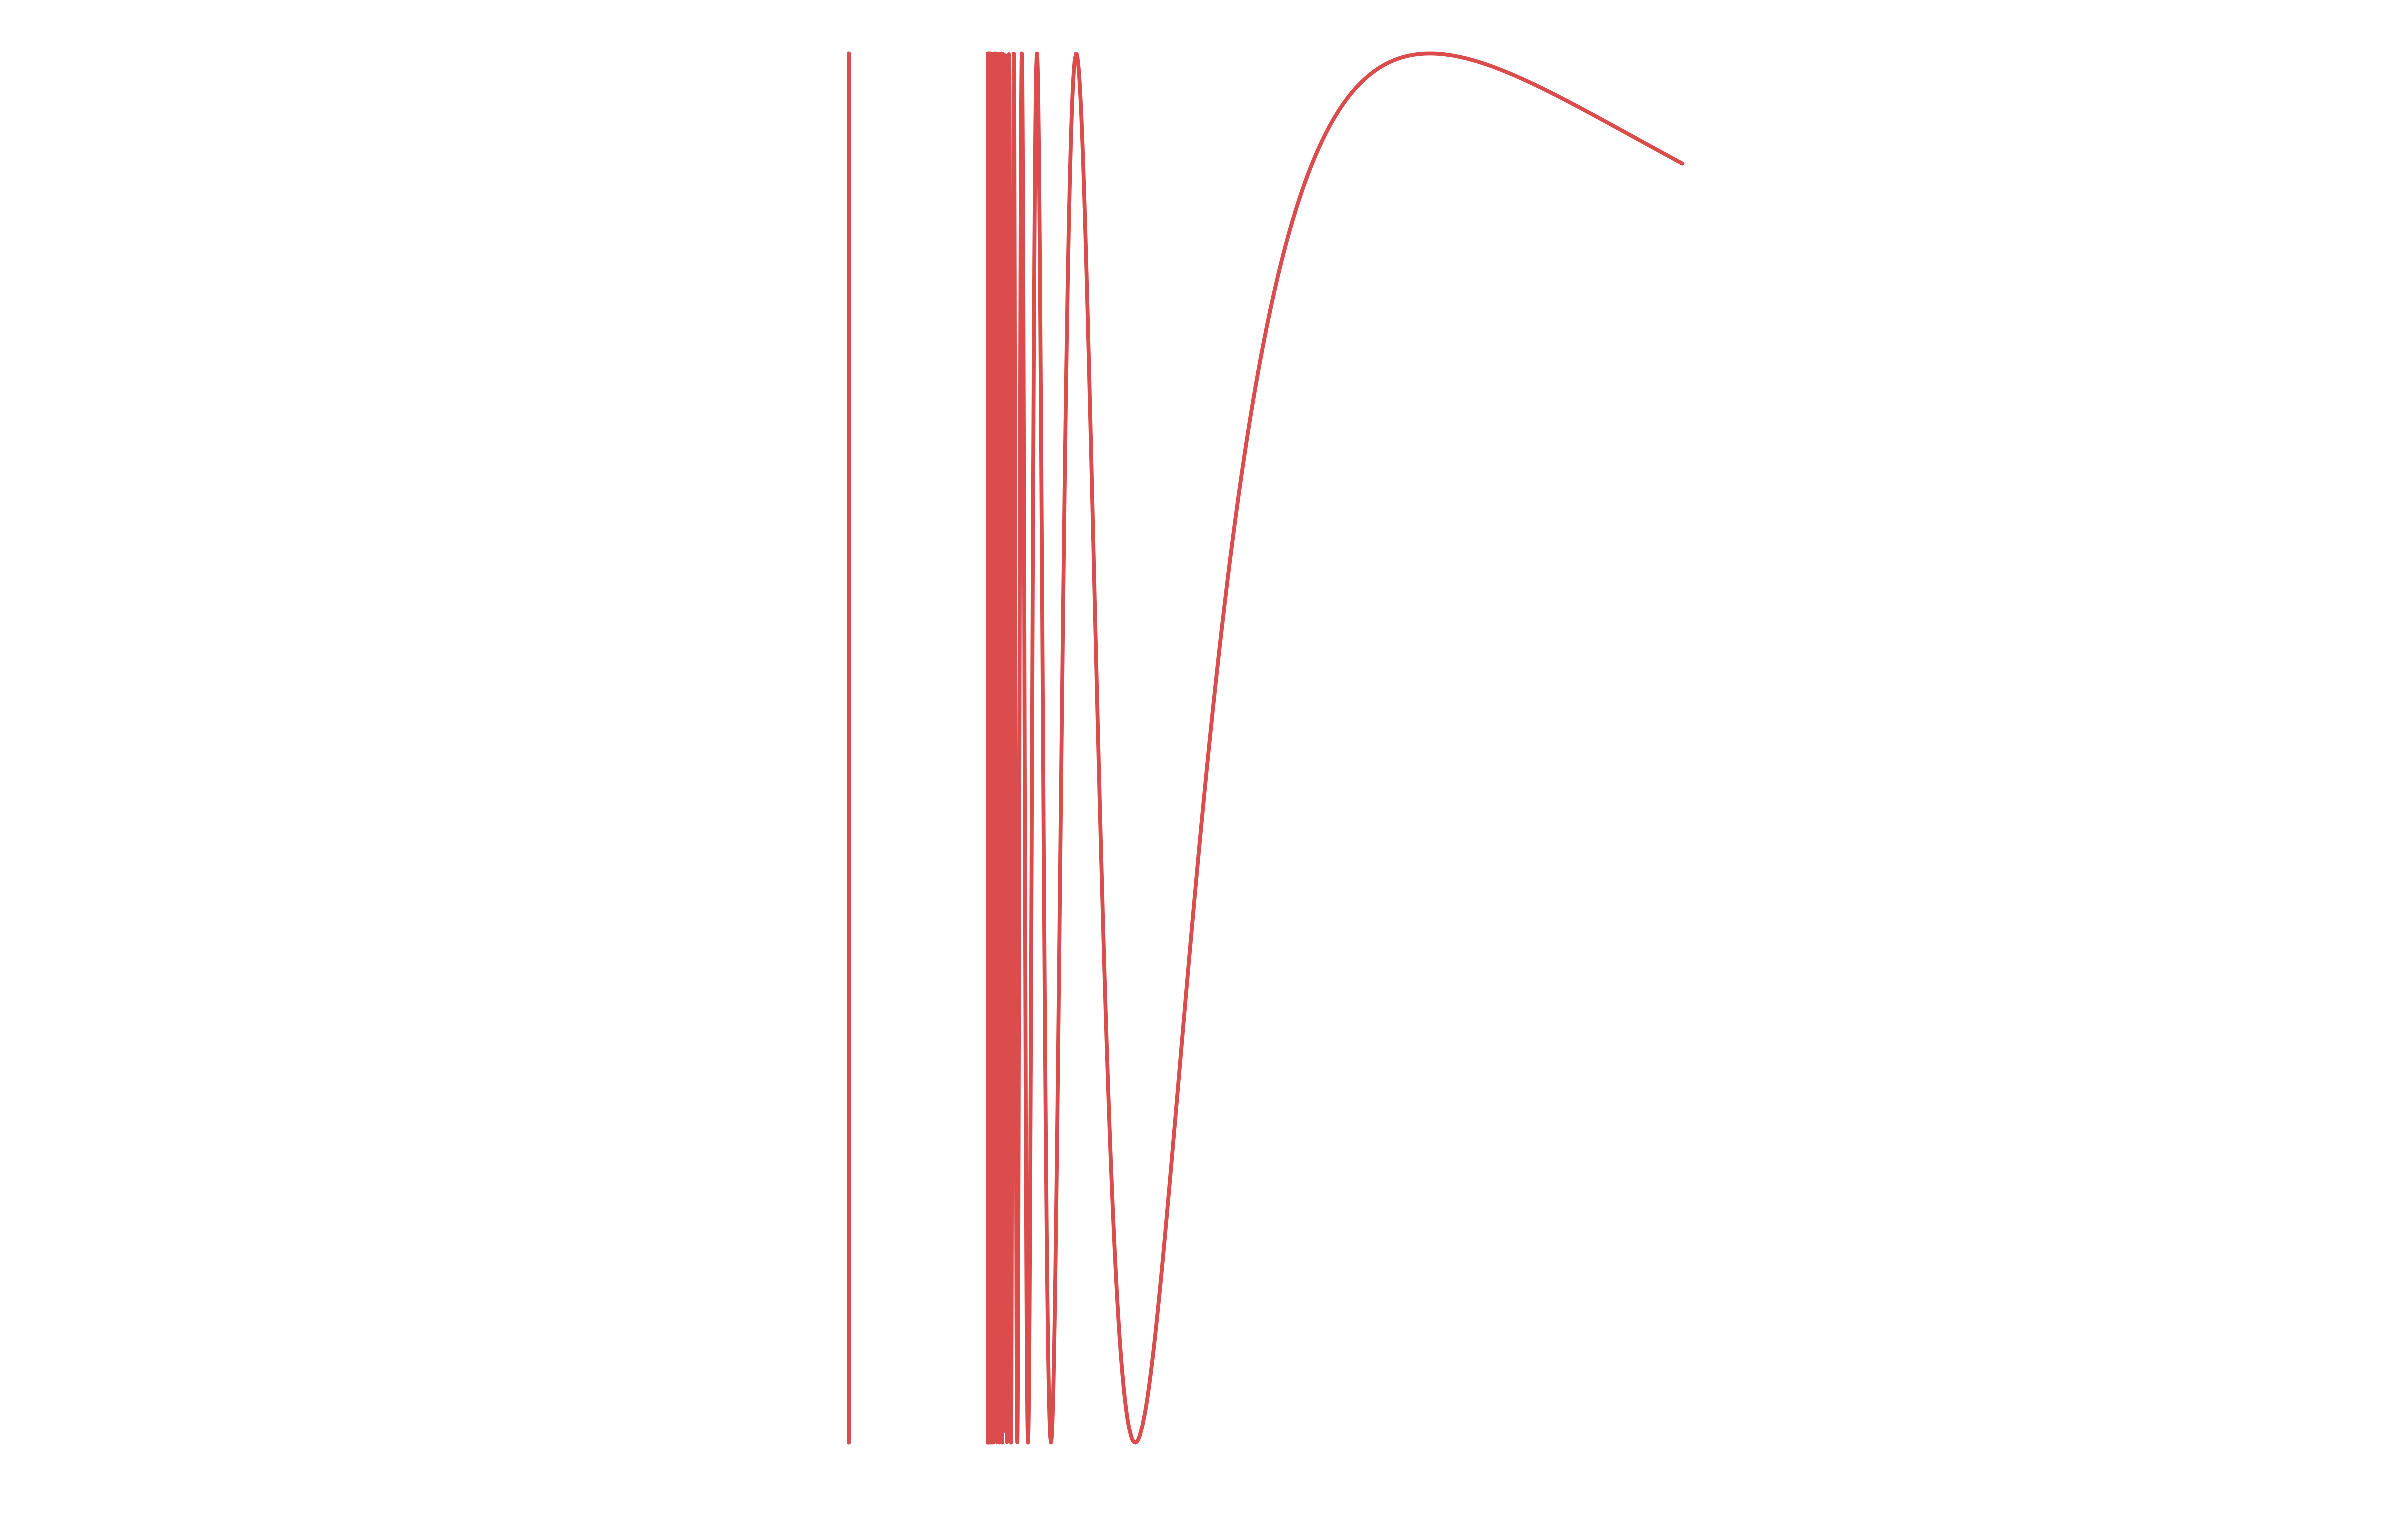
\includegraphics[scale = 0.2]{Figures/Chapter3/topologistsSineCurve.eps}
            \caption{The topologists Sine Curve, defined by $x \times \sin{\frac{1}{x}}$.}
            \label{fig_3.2}
        \end{figure}

        Let $S=\{x \times \sin{\frac{1}{x}}:0 < x \leq 1\}$. This is the image of the continuous map
        $x \rightarrow x \times \sin{\frac{1}{x}$ from $(0,1] \rightarrow \R^2$, Since $(0,1]$ is
            connected, then so is $S$. by theorem \ref{3.1.6}. We call $\cl{S}=S \cup (0 \times
            [-1,1])$ the \textbf{topologist's sine curve} (see figure \ref{fig_3.2}).

            Suppose that $f:[a,c] \rightarrow \cl{S}$ is a path begining at $0$ and ending at a
            point in  $S$. The set  $T=\{t \in \R:f(t) \in 0 \times [-1,1]\}$ is closed, so it has a
            largest element $b$. Then  $f$ is a path mapping  $b \rightarrow 0 \times [-1,1]$ and
            taking all other points to $S$. Suppose that  $[b,c]=[0,1]$ and let $f(t)=(x(t),y(t))$
            where $x(0)=0$, $x(t)>0$ and $y(t)=\sin{\frac{1}{x(t)}}$ for all $t>0$. For  $n \in
            \Z^+$, choose  $0<u<x(\frac{1}{n})$ such that $\sin{\frac{1}{u}}=(-1)^n$. By the
            intermediate value theorem, there are $0<t_n<\frac{1}{n}$ with $x(t_n)=u$. Then the
            sequence $\{t_n\} \rightarrow 0$, and $x(t_n)=(-1)^n$, which diverges; a contradiciton
            since $x(0)=0$ and $\{t_n\} \rightarrow 0$. Hence $\cl{S}$ is not path connected.

    \end{enumerate}
\end{example} 

%----------------------------------------------------------------------------------------
%	SECTION 1.1
%----------------------------------------------------------------------------------------

\section{Components and Local Connectedness.}

\begin{proposition}\label{3.3.1}
    Let $\sim$ be a relation defined on the topological space  $X$ by:  $x \sim y$ if there exists a
    connected subspace containing both  $x$ and  $y$. Then $\sim$ is an equivalence relation on
    $X$.
\end{proposition}
\begin{proof}
    Clearly, $x \sim x$. Now suppose that  $x \sim y$, then there is a connected subspace containing
    both  $x$ and  $y$, by definition,  $y \sim x$. Now suppose that  $x \sim y$ and  $y \sim z$.
    Then there are connected subspaces  $U$ and  $V$ with  $x,y \in U$,  $y,z \in V$. Since $y \in U
    \cap V$, by theorem \ref{3.1.4}, $U \cup V$ is a connected subspace with  $x,z \in U \cup V$.
    That is  $x \sim z$. 
\end{proof}

\begin{definition}
    Let $X$ be a topological space. Define an equivalence relation  $\sim$ on  $X$ by taking  $x
    \sim y$ if there is a onnected subspace of  $X$ containing  $x$ and  $y$. We call the
    equivalence classes of  $X/\sim$  \textbf{connected components} (or \textbf{components}) of
    $X$.
\end{definition}

%%----------------------------------------------------------------------------------------
%	SECTION 1.1
%----------------------------------------------------------------------------------------

\section{Compact Spaces.}

\begin{definition}
    A collection $\Ac=\{A_{\alpha}\}$ of subsets of a topological space $X$ is said to be a  \textbf{cover}, or a
    \textbf{covering} of $X$ if  $\bigcup{A}=X$. We call $\{A\}$ an \textbf{open cover} if each $A$
    is open in  $X$. If  $\{A'\}$ is a subcollection of $\Ac$ that also covers $X$, we call
    $\{A'\}$ a \textbf{subcover} of $X$.
\end{definition}

\begin{definition}
    We call a topological space $X$ \textbf{compact} if for every open cover of $X$, there is a
    finite subcover of $X$.
\end{definition}

\begin{example}
    \begin{enumerate}[label=(\arabic*)]
        \item     $\R$ is not compact. Consider the following cover of  $\R$:
            \begin{equation*}
                \Ac=\{(n,n+2):n \in \Z\}
            \end{equation*}
            however, there is no finite subcollection of $\Ac$ that is a subcover of  $\R$.

        \item The subspace $X=\{0\} \cup \{\frac{1}{n}: n \in \Z\}$ of $\R$ is compact. Let  $\Ac$
            be a cover of  $X$. There is a  $U \in \Ac$ with  $0 \in U$ and $U$ contains all but
            finitely many of the points  $ \frac{1}{n}$. Now choose for each $\frac{1}{n} \in
            \com{X}{U}$ an element of $\Ac$ $A_{n}$ containing it. Then for all $n$,  $\{A_n\}$ is
            finite and covers $X$.

        \item If  $X$ is a finite topological space, then it is compact, since every open cover of
            $X$ is finite.

        \item The interval  $(0,1]$ is not compact. The open cover $\Ac=\{(\frac{1}{n}, 1]: n \in
            \Z^+\}$ contains no finite subcollection of $\Ac$ that covers  $(0,1]$. Likewise,
            $(0,1)$ is not compact by the same argument. However, $[0,1]$ is compact.
    \end{enumerate}
\end{example} 

\begin{lemma}\label{3.4.1}
    Let $Y$ be a subspace of a topological space  $X$.  $Y$ is compact if and only if every open
    cover of  $Y$, by open sets of  $X$ has a finite subcover of $Y$.
\end{lemma}
\begin{proof}
    Suppose $Y$ is compact and let  $\{A_\alpha\}$ be a cover of $Y$ with  $A_\alpha$ open in  $X$
    for all  $\alpha$. Since  $\{A_\alpha\}$ covers $Y$, so does the collection  $\{A_\alpha \cap
    Y\}$, where $A_\alpha \cap Y$ is open in  $Y$ for all  $\alpha$. Since  $Y$ is compact, choose
    the finite subcollection  $\{A_i \cap Y\}_{i=1}^{n}$ to be a finite subcover of $Y$; i.e.
    $\{A_i \cap Y\}_{i=1}^{n} \subseteq \{A_\alpha\}$.

    Conversely, suppose that for every cover $\{A_\alpha\}$, open in  $X$, of  $Y$ that
    $\{A_\alpha\}$ contains a finite subcover of $Y$. Choose  $A_\alpha'=A_\alpha \cap Y$ for all
    $\alpha$; then $\{A_\alpha'\}$ is an open cover of $Y$. 
    By hypthesis, there is a finite subcover $\{A_i\}_{i=1}^n$, and by our assignment, we
    get that $\{A_i'\}_{i=1}^n \subseteq \{A_\alpha'\}$ is also a finite subcover of $Y$. Therefore
     $Y$ is compact as a subspace of  $X$.
\end{proof}

\begin{theorem}\label{3.4.2}
    Every closed subspace of a compact space is compact.
\end{theorem}
\begin{proof}
    Let $Y$ be a closed subspace of a compact space $X$. Let $\{A_\alpha\}$ be an open cover of $Y$
    with  $A_\alpha$ open in  $X$ for all  $\alpha$. Consider  $\{B_\alpha\}=\{A_\alpha\} \cup
    \com{X}{Y}$. Since $\{A_\alpha\}$ covers $Y$,  $\{B_\alpha\}$ covers $X$. Now take some finite
    subcollection  $\{B_i\}_{i=1}^n$. If it contains $\com{X}{Y}$, then just consider
    $\com{\{B_i\}}{(\com{X}{Y})}$. Then this collection is a finite subcover of $Y$.
\end{proof}

\begin{theorem}\label{3.4.3}
    Every compact subspace of a Hausdorff space is closed.
\end{theorem}
\begin{proof}
    Let $Y$ be a compact subsapce of a Hausdorff space  $X$. Choose  $x_0 \in \com{X}{Y}$ and for
    each $y \in Y$ choose disjoint neighborhoods  $U_y$ and  $V_y$ of  $ x_0$ and $y$ respectively.
    The collection  $\{V_y\}$ covers $Y$ by open sets in  $X$, hence there is a finite subcover, by
    theorem \ref {3.4.2}, $\{V_{y_n}\}$ of $Y$. Take  $V=\bigcup_{i=1}^n{V_{y_i}}$ to be open in
$X$, and take  $U=\bigcap_{i=1}^n{U_{y_i}}$ also open in $X$. Then  $Y \subseteq V$ and  $V \cap
U=\emptyset$; for take $z \in V$,  $z \in V_{y_i}$ for some $1 \leq i \leq n$. Hence  $z \notin
U_{y_i}$, so $z \notin U$. Then  $U$ is a neighborhood of  $X$, disjoint from  $Y$, making
$\com{X}{Y}$ open in $X$. Therefore  $Y$ is closed in  $X$.
\end{proof}

\begin{figure}[h] 
    \centering
    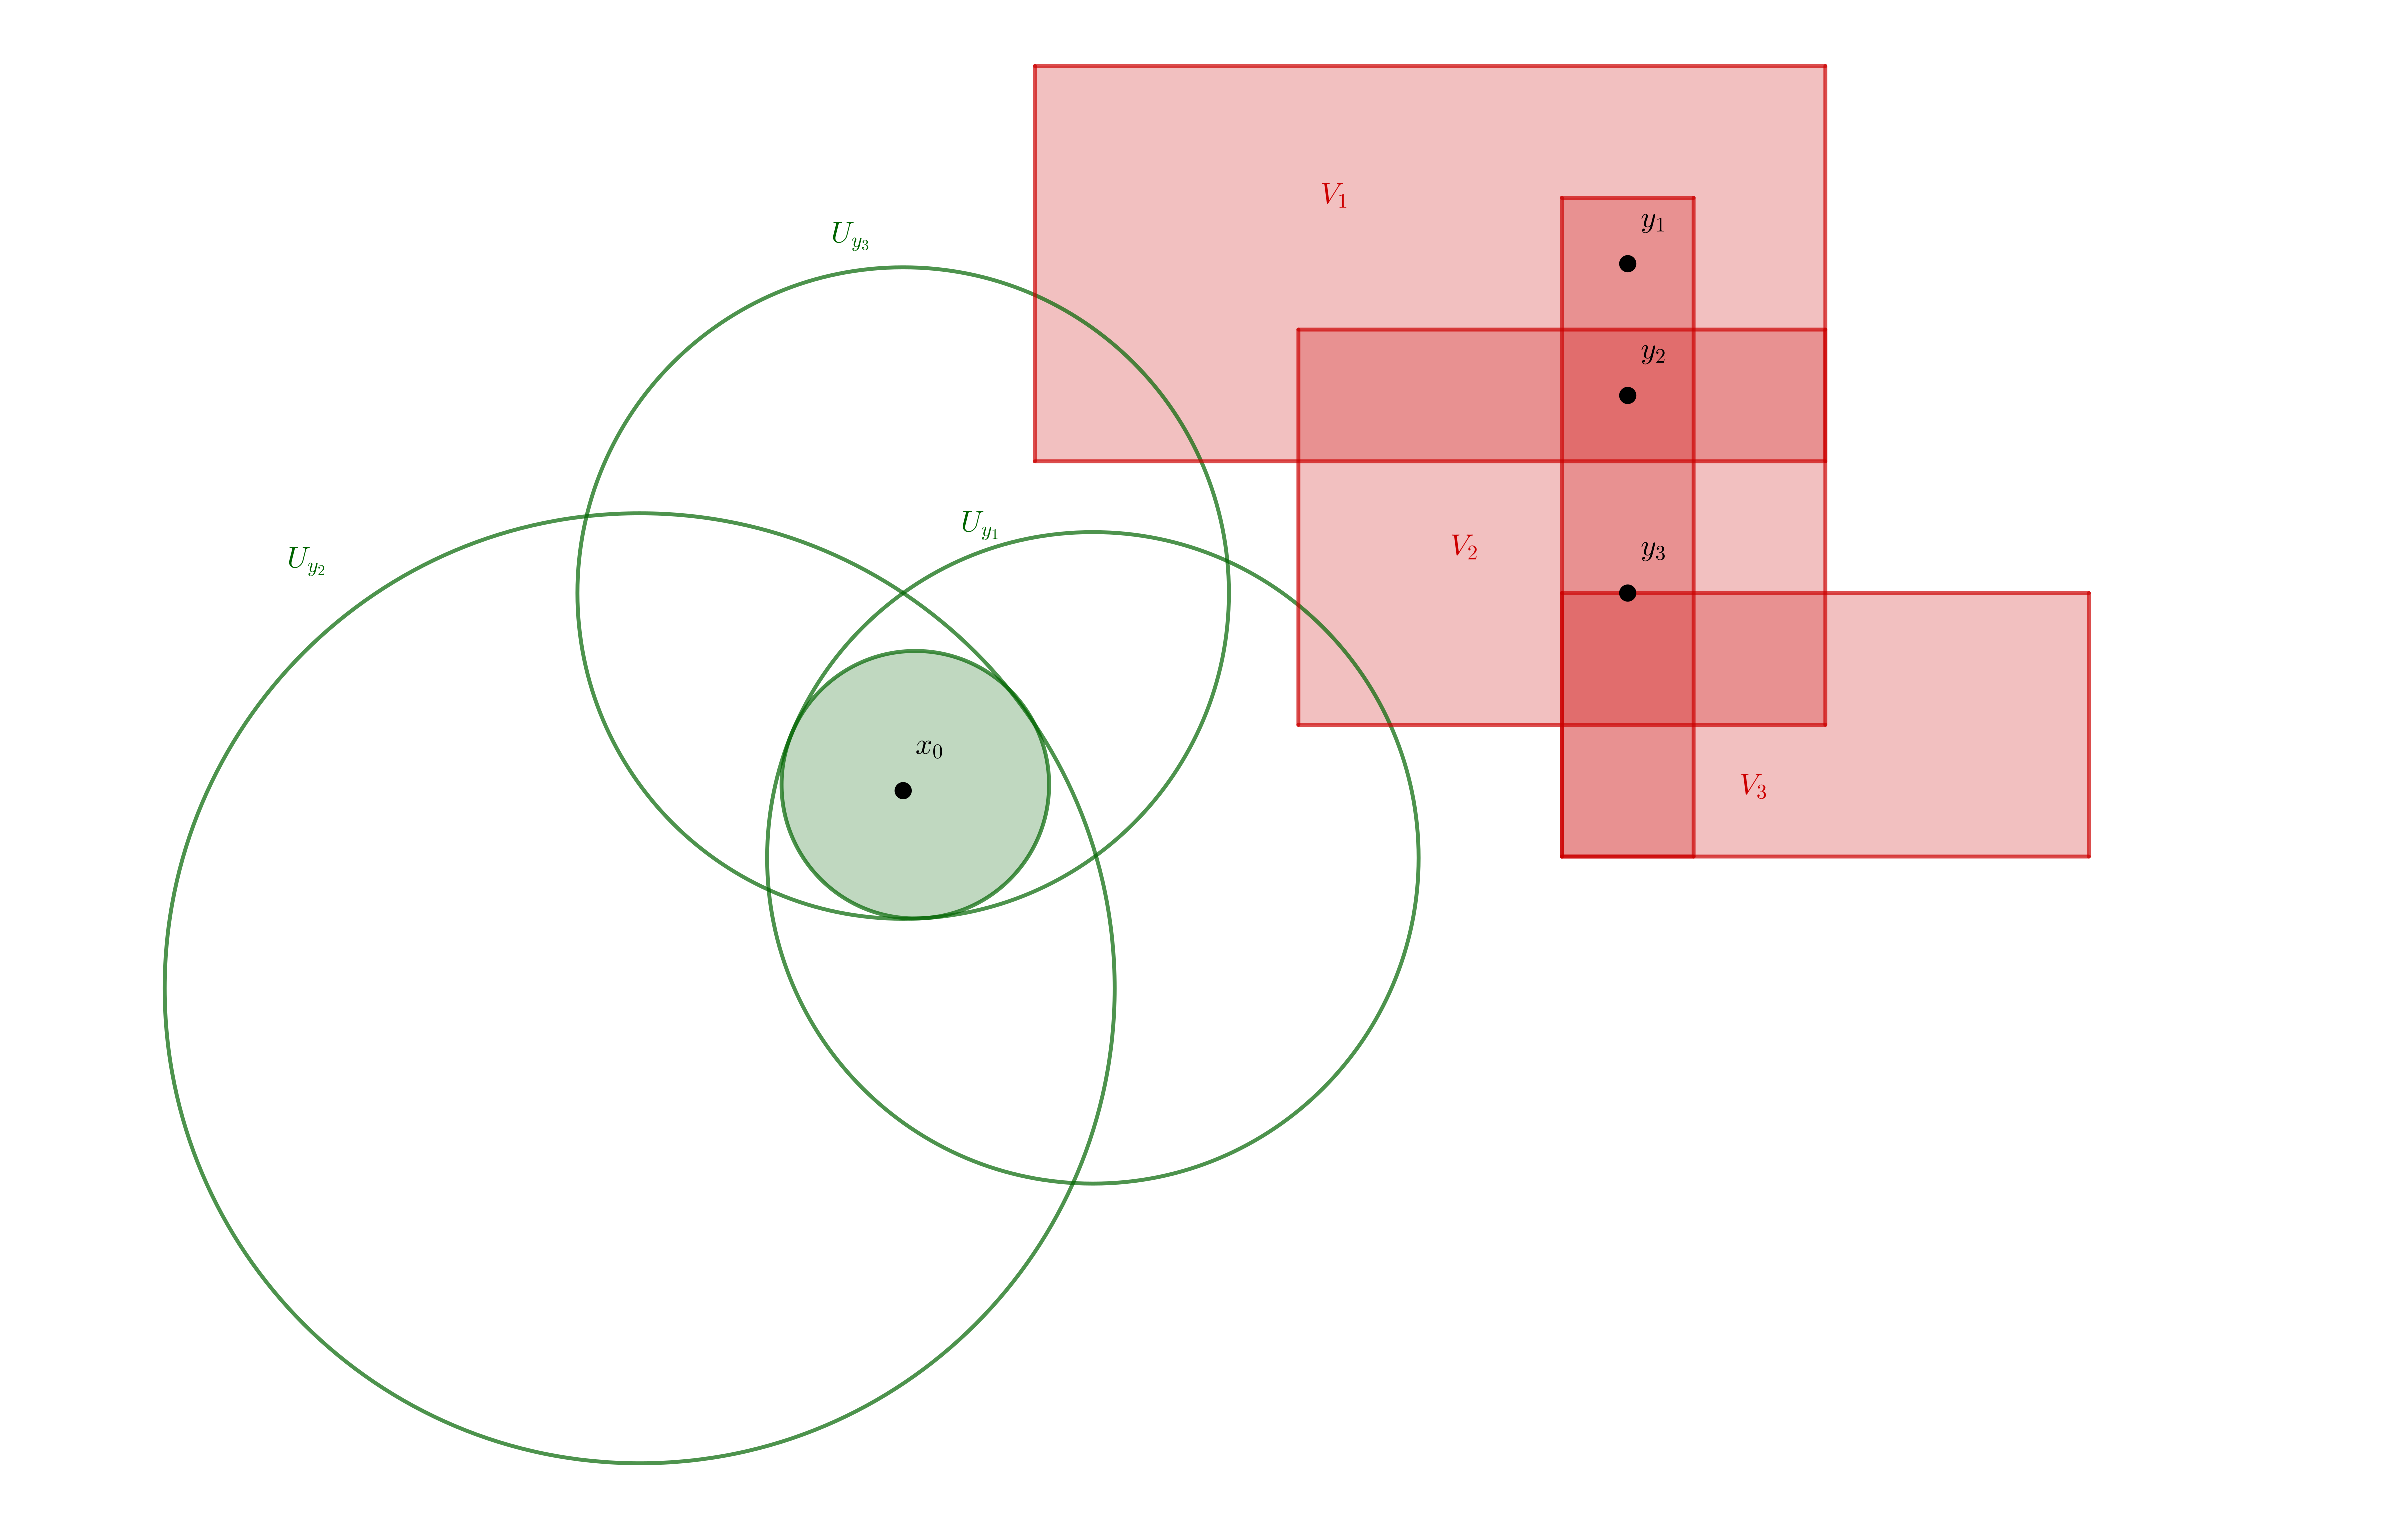
\includegraphics[scale=0.2]{Figures/Chapter3/compactHausdorff1.eps}
    \caption{}
    \label{fig_3.1}
\end{figure}

\begin{corollary}
    If $Y$ is a compact subspace of a Hausdorff space $X$, and  $ x_0 \in \com{X}{Y}$, then there
    exists opensets $U$ and  $V$ in  $X$ with  $ x_0 \in U$ and $Y \subseteq V$, respectively.
\end{corollary}

%%----------------------------------------------------------------------------------------
%	SECTION 1.1
%----------------------------------------------------------------------------------------

\section{Modules.}
\label{section1}

       				   % All the chapters goes here.
%\input{chapters/chapter4.tex}
%\input{chapters/chapter5.tex}
%\input{chapters/chapter6.tex}
%\input{chapters/chapter7.tex}
%555\input{chapters/capitulo5.tex}					   % If you want add this chapter remove the comment (%).
%%%%\input{chapters/chapter6.tex}                         % If you want add this chapter remove the comment (%).
%%%%%\input{chapters/Conclusion.tex}    				   % This is the last Chapter

%\appendix									           % End of the body of the thesis, begin of the appendices.
%\makeappendicespage		                           % Create a page with "APPENDICES" in the middle.

%% Appendix
%==========================================================================
\chapter{}
\label{AppA}
			           % This is the appendix A.
%% Appendix
%==========================================================================
\chapter{TITLE OF APPENDIX B}
\label{AppB}


Appendix B goes here.			           % This is the appendix B. For more appendices: \input{AppendixC.tex}
%%       Make List of References
%%%%%%%%%%%%%%%%%%%%%%%%%%%%%%%%%%%%%%%%%%%%%%%%%%%%%%%%%%%%%%%%
%% Note: I use BibTeX, but have coded in thebibliography environment
%%       to use for this example only.
%%%%%%%%%%%%%%%%%%%%%%%%%%%%%%%%%%%%%%%%%%%%%%%%%%%%%%%%%%%%%%%%


									% unstr is the same as
\begin{thebibliography}{1}
\bibliographystyle{plain}


\bibitem{sperber} A. Adolphson and S. Sperber. 
\newblock $p$-adic Estimates for Exponential Sums and the of Chevalley-Warning.
\newblock {\it Ann. Sci. Ec. Norm. Super.}, $4^{e}$ s\'erie,  {\bf 20}, 545--556, 1987.

\bibitem{acgmr} R. A. Arce-Nazario, F. N. Castro, O. E. Gonz\'alez, L. A. Medina and I. M. Rubio.
\newblock New families of balanced symmetric functions and a generalization of Cuscik, Li and P. St$\check{\mbox{a}}$nic$\check{\mbox{a}}$.
\newblock {\it Designs, Codes and Cryptography} {\bf 86}, 693--701, 2018.

\bibitem{ax} J. Ax.
\newblock Zeros of polynomials over finite fields. 
\newblock {\it Amer. J. Math.}, {\bf 86}, 255--261, 1964.

\bibitem{BCP} M. L. Bileschi, T.W. Cusick and D. Padgett.
\newblock Weights of Boolean cubic monomial rotation symmetric functions.
\newblock {\it Cryptogr. Commun.}, {\bf 4}, 105--130, 2012.

\bibitem{browncusick} A. Brown and T. W. Cusick.
\newblock Recursive weights for some Boolean functions. 
\newblock  {\it J. Math. Cryptology}, {\bf 6(2)}, 105--135, 2012.

\bibitem{cai} J. Cai, F. Green and T. Thierauf. 
\newblock On the correlation of symmetric functions.
\newblock {\it Math. Systems Theory}, {\bf 29}, 245--258, 1996.

\bibitem{canteaut} A. Canteaut and M. Videau.
\newblock Symmetric Boolean Functions.
\newblock {\it IEEE Trans. Inf. Theory} {\bf 51(8)}, 2791--2881, 2005.

\bibitem{Davis}
\newblock Philip Davis. Circulant Matrices.
\newblock Chelsea publishing, Second Edition,1994.

\bibitem{cgm3} F. N. Castro, O. E. Gonz\'alez and L. A. Medina.
\newblock Diophantine Equations With Binomial Coefficients and Perturbations of Symmetric Boolean Functions.
\newblock {\it IEEE Trans. Inf. Theory}, {\bf 64(2)}, 1347--1360, 2018.

\bibitem{cm1} F. N. Castro and L. A. Medina. 
\newblock Linear Recurrences and Asymptotic Behavior of Exponential Sums of Symmetric Boolean Functions. 
\newblock {\it Elec. J. Combinatorics}, 18:\#P8, 2011.

\bibitem{cm2} F. N. Castro and L. A. Medina. 
\newblock Asymptotic Behavior of Perturbations of Symmetric Functions.  
\newblock {\it Annals of Combinatorics}, 18:397--417, 2014.

\bibitem{cm3} F. N. Castro and L. A. Medina. 
\newblock Modular periodicity of exponential sums of symmetric Boolean functions.
\newblock {\it Discrete Appl. Math.} {\bf 217}, 455--473, 2017.

\bibitem{cms} F. N. Castro, L. A. Medina and P. St$\check{\mbox{a}}$nic$\check{\mbox{a}}$.
\newblock Generalized Walsh transforms of symmetric and rotation symmetric Boolean functions are linear recurrent.
\newblock {\it Appl. Algebra Eng. Commun. Comput.}, DOI 10.1007/s00200-018-0351-5, 2018.

\bibitem{ccms} F. N. Castro, R. Chapman, L. A. Medina, and L. B. Sep\'ulveda.  
\newblock Recursions associated to trapezoid, symmetric and rotation symmetric functions over Galois fields.
\newblock {\it Discrete Mathematics.},{\bf 341}, 1915--1931, 2018.

\bibitem{cusick4} T. W. Cusick. 
\newblock Hamming weights of symmetric Boolean functions.
\newblock {\it Discrete Appl. Math.} {\bf 215}, 14--19, 2016.

\bibitem{cusickArXiv} T. W. Cusick.
\newblock Weight recursions for any rotation symmetric Boolean functions.
\newblock {\it IEEE Trans. Inf. Theory}, {\bf 64}, 2962 - 2968, 2018.

\bibitem{cusickjohns} T. W. Cusick and B. Johns.
\newblock Recursion orders for weights of Boolean cubic rotation symmetric functions.
\newblock {\it Discr. Appl. Math.}, {\bf 186}, 1--6, 2015.

\bibitem{cusick2} T. W. Cusick, Y. Li, and  P. St$\check{\mbox{a}}$nic$\check{\mbox{a}}$.
\newblock Balanced Symmetric Functions over $GF(p)$.
\newblock {\it IEEE Trans. Inf. Theory}, {\bf 5}, 1304--1307, 2008.

\bibitem{cusickstanica} T.W. Cusick and P. St$\check{\mbox{a}}$nic$\check{\mbox{a}}$.
\newblock Fast evaluation, weights and nonlinearity of rotation symmetric functions.
\newblock {\it Discr. Math.}, {\bf 258}, 289--301, 2002.

\bibitem{dalaimaitrasarkar} D. K. Dalai, S. Maitra and S. Sarkar. 
\newblock Results on rotation symmetric Bent functions.
\newblock {\it Second International Workshop on Boolean Functions: Cryptography and
Applications, BFCA'06}, publications of the universities of Rouen and Havre, 137--156, 2006.

\bibitem{fengliu} K. Feng and F. Liu. 
\newblock New Results On The Nonexistence of Generalized Bent Functions. 
\newblock {\it IEEE Trans. Inf. Theory} {\bf 49},  3066--3071, 2003.

\bibitem{ggz} Y. Guo, G. Gao, Y. Zhao.
\newblock Recent Results on Balanced Symmetric Boolean Functions.
\newblock {\it IEEE Trans. Inf. Theory} {\bf 62 (9)}, 5199--5203, 2016.

\bibitem{hell} M. Hell, A. Maximov and S. Maitra. 
\newblock On efficient implementation of search strategy for rotation symmetric Boolean functions. 
\newblock {\it Ninth International Workshop on Algebraic and Combinatorial Coding Theory, ACCT 2004}, Black Sea Coast, Bulgaria,
2004.

\bibitem{hg} Y. Hu and G. Xiao.
\newblock Resilient Functions Over Finite Fields.
\newblock {\it IEEE Trans. Inf. Theory} {\bf 49},  2040--2046, 2003.

\bibitem{ims} E. J. Iona\c{s}cu, Thor Martinsen, Pantelimon St$\check{\mbox{a}}$nic$\check{\mbox{a}}$.
\newblock Bisecting binomial coefficients.
\newblock {\it Discrete Appl. Math.} {\bf 227} (2017) 70--83.

\bibitem{fspectrum} M. Kolountzakis, R. J. Lipton, E. Markakis, A. Metha and N. K. Vishnoi. 
\newblock On the Fourier Spectrum of Symmetric Boolean Functions.
\newblock {\it Combinatorica}, {\bf  29}, 363--387, 2009.

\bibitem{KScW} P.V. Kumar, R.A. Scholtz, and L.R. Welch. 
\newblock Generalized Bent Functions and Their Properties.
\newblock {\it J. Combinatorial Theory (A)}, {\bf 40}, 90--107, 1985.

\bibitem {licusick1} Y. Li and T.W. Cusick. 
\newblock Linear Structures of Symmetric Functions over Finite Fields.
\newblock {Inf. Processing Letters} {\bf 97}, 124--127, 2006.

\bibitem{licusick2} Y. Li and T. W. Cusick. 
\newblock Strict Avalanche Criterion Over Finite Fields.
\newblock {\it J. Math. Cryptology}  {\bf 1(1)}, 65--78, 2006.

\bibitem{llm}M. Liu, P. Lu and G.L. Mullen. 
\newblock Correlation-Immune Functions over Finite Fields.
\newblock {\it IEEE Trans. Inf. Theory} {\bf 44}, 1273--1276, 1998.

\bibitem{maxhellmaitra} A. Maximov, M. Hell and S. Maitra. 
\newblock Plateaued Rotation Symmetric Boolean Functions on Odd Number of Variables. 
\newblock {\it First Workshop on Boolean Functions:Cryptography and Applications, BFCA'05}, publications of the universities of Rouen and Havre, 83--104, 2005.

\bibitem{mitchell}  C. Mitchell.
\newblock Enumerating Boolean functions of cryptographic significance.
\newblock {\em J. Cryptology} {\bf 2} (3), 155--170, 1990.

\bibitem{mm1} O. Moreno and C. J. Moreno.
\newblock Improvement of the Chevalley-Warning and the Ax-Katz theorems.
\newblock {\it Amer. J. Math.}, {\bf 117}, 241--244, 1995.

\bibitem{mm} O. Moreno and C. J. Moreno.
\newblock The MacWilliams-Sloane Conjecture on the Tightness of the Carlitz-Uchiyama Bound and the Weights of Dual of BCH Codes.
\newblock {\it IEEE Trans. Inform. Theory}, {\bf 40},  1894--1907, 1994.

\bibitem{parkerpott} M. G. Parker and A. Pott. 
\newblock On Boolean functions which are bent and negabent.
\newblock {\it Proc. Int. Conf. Sequences, Subsequences, Consequences},
LNCS-4893, 9--23, 2007.

\bibitem{piequ} J. Pieprzyk and C.X. Qu.
\newblock Fast hashing and rotation-symmetric functions.
\newblock {\it J. Universal Comput. Sci.}, {\bf 5 (1)}, 20--31, 1999.

\bibitem{rp} C. Riera and M. G. Parker.
\newblock Generalized bent criteria for Boolean functions.
\newblock {\it IEEE Trans. Inform. Theory} {\bf 52} (9), 4142--4159, 2006.

\bibitem{fdegree} A. Shpilka and A. Tal.
\newblock On the Minimal Fourier Degree of Symmetric Boolean Functions.
\newblock {\it Combinatorica}, {\bf 88}, 359--377, 2014.

\bibitem{stanicamaitra} P. St$\check{\mbox{a}}$nic$\check{\mbox{a}}$ and S. Maitra. 
\newblock Rotation Symmetric Boolean Functions -- Count and Cryptographic Properties. 
\newblock {\it Discr. Appl. Math.}, {\bf 156}, 1567--1580, 2008

\bibitem{stanicamaitraclark} P. St$\check{\mbox{a}}$nic$\check{\mbox{a}}$, S. Maitra and J. Clark. 
\newblock Results on Rotation Symmetric Bent and Correlation Immune Boolean Functions. 
\newblock {\it Fast Software Encryption, FSE 2004}, Lecture Notes in Computer Science, {\bf 3017}, 161--177. SpringerVerlag, 2004.

\end{thebibliography}

\addcontentsline{toc}{extrachapter}{BIBLIOGRAPHY}%







%\bibliography{referencefiles/references.bib} 		% Use the References.bib file

%\backmatter %

%\biography{										% Add the Biography pages if you want.
%% Biography.tex

Here goes the Biography.

Use the file: \fn{Biography.tex}

%%%% CESAR ACEROS %%%% Biography %%%%%

%Cesar A Aceros was born in Dec, 23 of 1970 in Bucaramanga, Santander, Colombia. Cesar is son of Rodolfo Aceros Fajardo and Esperanza Moreno de Aceros. In October of 1995 receive the Electronic Engineer degree from the Pontificia Universidad Javeriana. He works in Conalvidrios S.A. the second in importance bottle glass factory in Colombia and later in August of 1996, he works at the Universidad Pontificia Bolivariana in Bucaramanga as a proffesor. In 2003 he left Colombia and start the M.S. studies at the University of Puerto Rico at Mayag\"uez. 


%%%% ALBERTO SANTANA %%%% Biography %%%%%

%was born on May 2$^{\rm nd}$, 1972, in San Germ\'an, Puerto Rico. Alberto is the son of Radam\'es Santana and N\'elida Vargas. In June 1995 he received his B.S.\ degree in chemistry from the University of Puerto Rico, Mayag\"uez Campus. In August of the same year, he started his graduate education. He worked under the supervision of Dr.\ Samuel P.\ Hern\'andez. Alberto spent more than two years doing research in the area of surface enhanced Raman spectroscopy (SERS). In June of 1998, Alberto received his second academic degree, a M.S.\ in chemistry from the same university.
%
%After doing experimental work, Alberto decided to continue his academic formation, but this time it would be in another area of chemistry. He came to the USA in January of 1998 and joined the Physical Chemistry Division of the Chemistry Department at the University of Florida. After completing his written and oral examinations, Alberto was admitted to the Ph.D.\ program and started his research on the theoretical and computational aspects of quantum molecular dynamics applied to surface chemistry under the supervision of Dr. David A. Micha. 
			
%}

%%%%%%%%%%%%%%%%%%%%%%%%%%%%%%%%%%%%%%%%%%%%%%%
%%  Create a General Audience Abstract      %%%
%%%%%%%%%%%%%%%%%%%%%%%%%%%%%%%%%%%%%%%%%%%%%%%

%\begin{simpleenv}{}{}{}{}%
%\pagestyle{empty}
%\begin{flushleft}
%\Title\\*[\BaseDiff\baselineskip]
%\FullName\\%
%(787) XXX-XXXX\\%
%Department of \Department \\%
%Chair: \Chair\\%
%Degree: \DegreeType\\%
%Graduation Date: \GradMonth~\GradYear%
%\end{flushleft}
%\GoDouble%
%% GeneralAudienceAbstract.tex


This is the general Audience Abstract.

Use the file: \fn{GeneralAudienceAbstract.tex}

%Density matrix theory is applied to the CO/Cu(001)
%adsorbate/substrate system to evaluate the nonlinear photodesorption yield of CO versus pulse fluence through model calculations. The dynamics of molecular photodesorption from a metal surface is described by the nonlinear optical response resulting from the interaction of a femtosecond pulsed laser with a metal surface. Our formalism uses the Liouville-von Neumann equation, with an effective hamiltonian which includes the effects of energy dissipation into the metal. The nonlinear response of the substrate to femtosecond excitation is taken into account by solving modified optical Bloch equations with relaxation terms to account for the effects of energy dissipation. Our previous density matrix treatment has been extended to include several quantum states, and to treat rotational motions of the desorbing molecule. Results for intense lasers including chirping at pulse wavelengths around 620 nm have also been obtained.

%\end{simpleenv}

	
				                   % This file create the Bibliography, Biography and general abstrac for the thesis.
\end{document} 